\documentclass{egpubl}
\usepackage{eurovis2026}
\STAREurovis
\CGFccbyncnd
\usepackage[T1]{fontenc}
\usepackage[utf8]{inputenc}
\usepackage{microtype}
\emergencystretch=1em
\usepackage{dfadobe}
\usepackage{cite}
\BibtexOrBiblatex
\electronicVersion
\PrintedOrElectronic
\usepackage[pdftex]{graphicx}
\paperwidth=210mm
\paperheight=297mm
\usepackage{egweblnk}
\usepackage{booktabs}
\usepackage{array}
\usepackage{tabularx}
\usepackage{xcolor}
\newif\ifdraftnotes
\draftnotesfalse % Change to \draftnotesfalse to hide editorial notes.
\newcommand{\draftnote}[1]{\ifdraftnotes\par\smallskip{\small\color{blue!55!black}\noindent\textbf{Revision note:} #1\par}\smallskip\fi}
\newcommand{\plan}[1]{\par\noindent\textbf{Outline.} #1\par}
\title[From Hairballs to Hypotheses]{From Hairballs to Hypotheses: A Survey of AI-Assisted Visual Analytics in the Life Sciences}
\author[Chukhman et al.]
{\parbox{\textwidth}{\centering
Morris Chukhman$^{1,2}$,
Amira Kefi$^{1}$,
Nicole M. Chukhman$^{3}$,
Silvio Rizzi$^{1,4}$,
Vinayakumar Chalil Karintha$^{5}$\,
and Angus Forbes$^{6}$\\[1ex]
{\small
$^{1}$University of Illinois at Chicago, Chicago, IL, USA\\
$^{2}$St. Luke's University Health Network, Stroudsburg, PA, USA \\
$^{3}$University of Wisconsin - Madison, Madison, WI, USA \\
$^{4}$Argonne National Laboratory, Lemont, IL, USA \\
$^{5}$UST, Thiruvananthapuram, Kerala, India \\
$^{6}$NVIDIA, Santa Clara, CA, USA \\
}
}
}

\begin{document}
\maketitle
\begin{abstract}
Life-science visual analytics supports scientists in exploring biological data, interpreting patterns, and developing hypotheses. However, displaying dense biological relationships creates visual “hairballs” when overlapping connections make individual relationships and broader patterns difficult to discern. To examine how systems support these activities we present an Assistance × Visualization Modality framework for classifying life-science visual analytics systems and comparing how they support scientific analysis. The framework connects computational mechanisms and display environments to five task groups: navigation, comparison, selection, sensemaking, and collaboration. We examine the locus of analytic agency, here understood as how initiative and control over analytical actions are distributed between scientists and software, and its implications for interpreting and validating results. We screened titles and available abstracts, identifying 9,505 candidates for further assessment. We then selected systems with contrasting forms of computational assistance and examined their full-text reports to assess survey eligibility, place them within the framework, identify their computational mechanisms, and determine how they were evaluated. These comparisons distinguish configuring an analysis pipeline from training a model, organizing a visual representation from optimizing it, and interrogating predictions from assessing their supporting evidence. These distinctions inform evaluation of both computational performance and scientists’ ability to inspect, correct, and interpret the results. This framework helps researchers compare assistance mechanisms and display environments for particular scientific tasks by clarifying software functions, decisions that remain with scientists, and evaluation questions relevant to assessing analytical benefits.

\end{abstract}
\section{Introduction}
\label{sec:introduction}
Understanding biological systems requires reasoning across relationships and scales: from molecular interactions and cellular organization to neural connectivity and coordinated physiological processes. Visual analysis makes these relationships available for inspection, yet dense networks can collapse into ``hairballs'' in which connectivity is visible while scientifically meaningful structure remains difficult to discern. Analysts must determine which relationships matter, move between local detail and broader context, compare competing patterns, and connect visual observations to biological hypotheses. Supporting this work requires decisions about what to represent, aggregate, prioritize, and inspect next. How these decisions are made, and how they are distributed between scientists and computational systems, shapes both the course of exploration and the evidence available for scientific interpretation.

Computational assistance participates in these decisions by transforming representations, directing attention, and supporting the selection and execution of analytic actions. Clustering, aggregation, layout, and dimensionality reduction can make complex relationships tractable for inspection. Adaptive mechanisms can use interaction history or task context to recommend actions or reorganize what is shown. Conversational interfaces allow scientists to specify requests in language and, in more elaborate workflows, delegate sequences of operations for subsequent inspection. These mechanisms involve different forms of computational participation, rather than successive stages in which newer techniques necessarily provide better assistance. Established algorithms and newer AI methods are relevant here because of the work they perform within analysis. Their interventions shape what scientists encounter, which actions become available, and which decisions remain subject to direct human judgment.

Examining this distribution of responsibility requires bringing together several perspectives in the review literature. Surveys of biological network visualization address the representations and interactions through which biological relationships become accessible~\cite{Ehlers2025}. Broader network-visualization surveys connect techniques with analytical tasks~\cite{Filipov2023Roadmap}, while reviews of immersive analytics and immersive network analysis examine visualization in spatial interaction environments~\cite{Fonnet2019ImmersiveAnalytics,Joos2025VisNetIA}. These perspectives provide a basis for examining representations, tasks, and interaction environments. Comparing computational assistance across them also requires attention to the analytical work performed by software and the decisions retained by scientists.

Systems supporting related scientific tasks can differ substantially in what computation does and which decisions remain with scientists. A computed layout, a recommendation based on user feedback, and an operation generated through language may appear in similar views while assigning different choices and verification responsibilities to scientists. Comparing these approaches requires connecting their computational mechanisms and display environments to the analytical actions they support. This connection is needed to examine design alternatives and determine what evidence would establish their analytical benefits. We therefore distinguish implemented capabilities, proposed uses, and findings supported by evaluation.

To support these comparisons, we present the Assistance $\times$ Visualization Modality framework, which organizes systems by their computational assistance mechanisms and display environments. The framework connects these dimensions to five task groups: navigation, selection, comparison, sensemaking, and collaboration. Across these tasks, scientists and computation take different roles in initiating and directing analytical actions. We examine this distribution through the \emph{locus of analytic agency}, here understood as how initiative and control over analytical actions are distributed between scientists and computation, and consider its implications for interpreting and validating results. The contribution is a life-science application of existing agency and automation concepts: we relate specific analytical decisions to computational mechanisms, display environments, and the evidence needed to assess scientific interpretation. Together, the framework and the analysis of agency organize comparisons of design alternatives, scientists' decisions, and the evidence needed to assess analytical benefits.

This STAR focuses on the interactive visual analysis of dense relationships, derived structures, and multiscale biological context in the life sciences. We examine approaches in terms of their implemented computational mechanisms, evaluated benefits, and proposed capabilities. Although the title foregrounds AI-assisted systems, the review also includes established non-learning algorithms when they make a substantive contribution to interactive visual analysis.

\paragraph*{Research questions.}
We address the following four research questions:
\begin{enumerate}
\item[\textbf{RQ1.}] What recurring analytic tasks characterize computationally assisted visual analysis in the life sciences?
\item[\textbf{RQ2.}] How do different forms of computational assistance participate in those tasks and redistribute analytic agency between human and system?
\item[\textbf{RQ3.}] How do visualization modalities condition the form, effectiveness, and consequences of that assistance?
\item[\textbf{RQ4.}] How are these systems evaluated, and what benefits, limitations, risks, and design obligations emerge as computational participation becomes more consequential?
\end{enumerate}

\paragraph*{Contributions.}
This STAR contributes (1) a documented systematic search and screening workflow, followed by full-text assessment of selected systems to compare different forms of computational assistance in relational and multiscale life-science analysis; (2) an Assistance $\times$ Visualization Modality framework that organizes systems by computational mechanisms, display environments, and five scientific task groups; (3) an analysis of how scientists and computation share initiative and control over analytical actions, and the implications for interpretation and validation; and (4) a comparison of how existing systems have been evaluated, the benefits and limitations supported by those evaluations, and questions requiring further research.

Section~\ref{sec:methodology} describes the review methodology. Section~\ref{sec:foundations} establishes the conceptual foundations. Sections~\ref{sec:tasks}--\ref{sec:modality} examine analytic tasks, computational assistance, and visualization modalities; Section~\ref{sec:evaluation} compares evaluation methods and reported findings. Section~\ref{sec:challenges} discusses research challenges and opportunities, and Section~\ref{sec:conclusion} concludes.

\section{Review Methodology}
\label{sec:methodology}
The review combined broad bibliographic search, automated title-and-abstract screening and provisional classification, and full-text assessment of selected systems. Candidate labels guided discovery; report evidence supported system placements and six detailed comparisons involving twelve systems. Figure~\ref{fig:study-selection-flow} distinguishes records, reports, systems, and placements.

\subsection{Review Scope and Eligibility}
\label{sec:methodology-scope}
The scope is computationally assisted visual analysis of relational and multiscale life-science data. Screening used \emph{bibliographic records} containing titles, available abstracts, and metadata. Full-text assessment used \emph{research reports} to assess the \emph{systems} they describe; several reports can concern one system. At least one system in a report must satisfy all five criteria:

\begin{description}
\item[E1: Life-science application.] Supports analysis, understanding, monitoring, decisions, discovery, or scientific practice in a life-science or closely related domain; training, teleoperation, or presentation alone is insufficient.
\item[E2: Relational or multiscale relevance.] Concerns explicit networks or relationships derived from spatial, temporal, multivariate, image, lineage, similarity, or multiscale data; a network diagram is not required.
\item[E3: Visual-analytics component.] A human uses an interactive or analytically meaningful visual representation to inspect, validate, steer, compare, or interpret data or results; illustration alone is insufficient.
\item[E4: Substantive computational assistance.] A mechanism contributes nontrivially to that workflow, such as clustering, layout, aggregation, annotation, ranking, prediction, or interpreted operations; rendering, pan/zoom, direct parameter entry, or lookup alone does not qualify.
\item[E5: Human analytic relationship.] People inspect, direct, validate, interpret, supervise, correct, or decide from the assisted process; manual control of every operation is not required.

\end{description}

Surveys and general interaction studies provide background and additional discovery routes. Eligibility assessment focuses on reports describing systems and their analytical workflows. Each criterion is assessed using evidence about the same system.

\subsection{Sources and Search Strategy}
\label{sec:methodology-search}
Sources were PubMed, Europe PMC, Semantic Scholar, IEEE Xplore, ACM Digital Library, a local arXiv snapshot, and prior-survey materials. Five overlapping query families covered relational visualization, assisted analysis, interactive systems, nondesktop environments, and conversational analysis. Each combined life-science terms with system, relationship, assistance, or environment terms, including assistance-neutral expressions to retrieve methods without an AI label. Provider syntax and searched fields are documented in the query specifications.

The documented retrieval cutoff was 20 September 2026, with no restriction on the earliest publication date. arXiv identification used a local snapshot containing 3,164,528 records and yielded 958 distinct matches across the query families. Observed snapshot metadata updates extended through 11 September 2026. The snapshot's coverage is considered separately from the cutoff used for the other retrieval routes.

Additional records came from Ehlers-associated working materials, Joos-associated companion material, and a reconstruction of Fonnet and Pri\'e's bibliography, contributing 816, 146, and 207 source occurrences, respectively.~\cite{Ehlers2025,Joos2025VisNetIA,Fonnet2019ImmersiveAnalytics} These records entered the screening workflow alongside database results. The source inventory retains their provenance and distinguishes confirmed survey members, unconfirmed entries, and background references.

\subsection{Deduplication and Source Provenance}
\label{sec:methodology-deduplication}
Deduplication consolidated 187,446 source occurrences into 140,959 bibliographic records using normalized DOI keys, or exact normalized titles when DOIs were absent. Records with and without DOIs remained separate when title agreement was insufficient. Source occurrences and identity decisions were retained, including 50 links between related publication versions. Reports describing the same system were grouped during full-text assessment. The accompanying methods supplement details the identity rules.

\subsection{Title-and-Abstract Screening}
\label{sec:methodology-screening}
Automated screening assessed E1--E5 from titles, available abstracts, and evidence identifiers using the OpenAI Responses API (\texttt{gpt-5.6-luna}, medium reasoning, default service tier, no inference-time browsing or tools). Responses were checked against supplied identifiers and outcomes recomputed locally. \emph{Advance} required support for all five criteria; \emph{Excluded} required evidence against at least one; \emph{Defer} marked insufficient evidence for either decision. Surveys remained background/discovery material, and infrastructure reports were assessed by their described analytical workflow.

Of the 140,959 deduplicated records, 140,810 received valid machine-assisted screening outcomes: 9,505 Advance, 83,258 Defer, and 48,047 Excluded. The remaining 149 records comprise 110 reserved pilot/calibration records, 35 technical failures, and four ambiguous requests that were not resubmitted. Among the excluded records, 10,460 also carried a background-literature flag indicating potential value for context or discovery. This flag is a designation within the excluded set. All 9,505 advanced records proceeded to candidate classification.

\begin{figure*}[t]
\centering
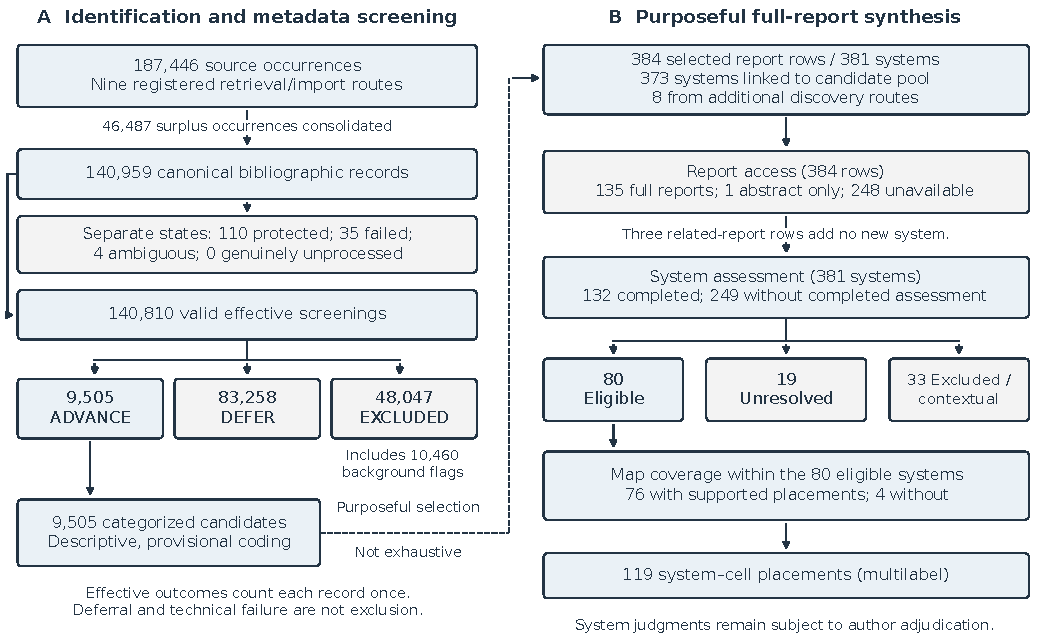
\includegraphics[width=\textwidth]{figures/figure1_selection_flow_119.pdf}
\caption{Identification, screening, and selected-system assessment, reconciled through 26 September 2026. Panel A counts source entries and deduplicated bibliographic records; Panel B distinguishes selected publication entries from the software systems they describe. The dashed handoff denotes selection of systems for detailed assessment. Eight systems entered through coauthor or bounded map-expansion routes without an exact link to the candidate pool. Related reports explain the difference between 135 accessible publication entries and 132 completed system assessments. Multilabel placements are not additional systems. Counts distinguish retrieved records, selected reports, assessed systems, and supported framework placements.}
\label{fig:study-selection-flow}
\end{figure*}

\subsection{Candidate Classification}
\label{sec:methodology-synthesis}
All 9,505 advanced records were provisionally classified from titles and available abstracts using the task, assistance, and modality definitions in Section~\ref{sec:foundations}. Labels could coexist and were recorded as Present, Absent, or Uncertain. These labels guided discovery and selection; supported system-level placements required report evidence for the actual mechanism--environment relationship. The accompanying methods supplement provides the classification contract and candidate co-occurrence table.

\subsection{Full-Text Assessment and Detailed Comparisons}
\label{sec:methodology-assessment}
Systems were selected to compare assistance mechanisms and improve coverage of sparse framework combinations. Six purpose-specific sets contained 20, 18, 50, 200, 24, and 72 report identities. Initial anchors and coauthor reports established comparison cases; bounded queues then prioritized coverage, mechanism and evaluation evidence, and contrasting cases. Software ranked the preliminary shortlist for the 50-entry set, but its final nominations were a separately specified list. The 200-entry queue was selected deterministically by high-precision workflow signal, coverage-rationale class, likely open access, metadata score, and canonical identifier. Software reconciled 25 provisional sparse-cell nominations to 24 entries. The final pass enumerated every exact Present-labelled candidate in three specified cells; scores determined access order, not inclusion. Selector identities and some within-priority rules for the static shortlists are not recorded. The accompanying methods supplement gives the rules, limits, and provenance distinctions for each set.

Assessment used accessible English-language reports to check eligibility, implemented mechanisms, task and modality labels, and evaluation methods and findings. Source passages documented inputs, operations, human intervention, and opportunities to inspect or revise results. Implemented capabilities, measured outcomes, and proposed extensions were recorded separately. The report--system crosswalk traces selection routes, identities, report versions, access, and outcomes.

The selected set comprised 384 publication entries representing 381 systems. Of these, 376 publication entries and 373 systems have exact links to the candidate pool; eight systems were identified through coauthor suggestions or additional searches for framework coverage. Full text was accessible for 135 publication entries, one entry supplied only an abstract, and 248 entries lacked accessible full text. Three accessible entries described related publications about systems already represented, yielding 132 completed system assessments and 249 systems without completed assessments.

Reports describing the same system were grouped using the retained identity crosswalk. Assessments recorded report versions, source passages, and qualifications for each placement. Of the 132 assessed systems, 80 were eligible, 19 remained scientifically unresolved, and 33 were excluded or retained for context. Seventy-six eligible systems supported 119 system--cell placements in Figure~\ref{fig:assistance-modality-map}; four eligible systems lacked a supported placement. A system may occupy several cells because different mechanisms and display environments can coexist. The lead author reviewed and confirmed the placements reported in Figure~\ref{fig:assistance-modality-map}.

A targeted assessment also examined candidate combinations in Immersive--Desktop/Planar, Immersive--Large Display, and Adaptive--Large Display. The 144 candidate memberships resolved to 131 records and 129 system groups, representing 142 distinct system--cell cases. Thirty cases were assessed from full-text reports: 28 lacked support for the proposed placement and two remained unresolved. The other 112 cases were access-limited. This assessment established no additional placements.

Twelve systems were selected for six detailed comparisons to examine how different computational contributions support related analytical work and distribute decisions between scientists and computation. For example, RNA-SeqEZPZ and Facetto illustrate the distinction between configuring an analysis pipeline and teaching a classifier through labeled examples. Compressed Adjacency Matrices and Flud illustrate analyst-controlled organization of a representation versus crowd-assisted optimization of its layout. RetainVis and MediSyn distinguish inspecting model predictions from assessing evidence supporting or contradicting a biomedical interpretation.

Selection considered the availability of reports documenting the mechanisms, human intervention, and evaluation. For each comparison, source passages established the actions performed by computation, the decisions retained or supplied by scientists, and the opportunities to inspect and revise results. These differences informed the evaluation questions developed in Section~\ref{sec:evaluation}. Selection for detailed comparison complemented the broader selection for assistance--modality coverage.

\subsection{Methodological Limitations}
\label{sec:methodology-limitations}
Search coverage depends on provider indexing, query terminology, and the arXiv snapshot's available metadata. The review therefore provides broad candidate discovery and selected-system comparisons rather than an exhaustive enumeration of eligible software. Prior-survey imports add retrieval routes, but coverage of references beyond those imports was not established through systematic recursive citation searching.

Advancement required explicit analytical evidence in titles and abstracts. This favors well-described systems and can defer eligible work with incomplete metadata. Full-text access further affects which systems can be assessed. Selection for framework coverage and detailed comparison supports examination of mechanisms; prevalence estimates would require a different sampling design. The crosswalk traces selected entries, but does not provide a record-by-record reason for leaving every other candidate unselected.

Automated screening and provisional classification were not independently validated across the entire candidate pool. Consequently, the false-exclusion rate, missed eligible systems among deferred records, and pool-wide classification reliability remain unknown. Author confirmation of selected framework placements checks those reported relationships; it cannot establish the accuracy of screening decisions for unreviewed records. Software checks and source verification support consistency and traceability. An independent, stratified review of Advance, Defer, and Excluded records would be needed to estimate screening errors and agreement.

Evaluation studies differ in tasks, datasets, participants, and measures. We compare the benefits and limitations supported within each study's conditions; these heterogeneous findings do not support a pooled effect estimate. The framework's usefulness for researchers has also not been independently evaluated.

\subsection{Supplementary Materials and Use of Generative AI}
\label{sec:methodology-materials}
The software implementing search, deduplication, screening, and evidence management is available at \url{https://github.com/iMammal/h2h-lit-pipeline}. The versioned reproducibility supplement, containing research data, evidence tables, and scripts for regenerating the reported tables and figures, is archived at \url{https://doi.org/10.5281/zenodo.23084434}.

The supplement contains provider-specific query specifications in \texttt{queries/}, retrieval and prior-survey import provenance in \texttt{identification/}, and screening and coding prompts, protocols, and execution settings in \texttt{prompts/}, \texttt{protocols/}, and \texttt{screening/}. The artifact inventory identifies included files and inputs retained outside the public supplement. Raw provider responses, the complete registered corpus, and copyrighted research reports are not redistributed.

\paragraph*{Use of generative AI.}
\label{sec:ai-disclosure}
OpenAI ChatGPT and Codex assisted with literature-processing software, evidence extraction and organization, system comparisons, manuscript drafting and revision, and preparation of LaTeX, tables, and figures. Automated screening and provisional classification used the Responses API as described in Section~\ref{sec:methodology-screening}. Google Gemini contributed preliminary calibration judgments. Checks included software tests, verification of record identities and source passages, deterministic recomputation of screening outcomes, citation checks, and inspection of rendered figures and documents. Reproduced interface images were extracted or cropped from their cited sources. The lead author reviewed all AI-generated content incorporated into the manuscript. The authors retain responsibility for its interpretation, accuracy, attribution, and final content.

\section{Conceptual Foundations: Tasks, Assistance, Modality, and Analytic Agency}
\label{sec:foundations}

We compare assisted visual analytics systems by describing the scientific tasks they support, their computational contributions, and their interaction environments. Tasks identify the analytical purpose, assistance describes the computational mechanisms, and visualization modality describes the environment through which scientists view and interact with the analysis. We examine the locus of analytic agency within these workflows: who initiates, directs, interprets, and corrects particular actions. These descriptions organize our comparisons of systems supporting related analytical work and help identify the evidence relevant to their claimed benefits. This section introduces the vocabulary used in those comparisons, beginning with the relationships and scales encountered in life-science data.

Established techniques such as clustering, dimensionality reduction, and graph layout qualify through their substantive role in an analytical workflow; their inclusion does not imply that these methods are new or require learning-based AI.

\subsection{Relational and Multiscale Life-Science Analysis}
\label{subsection:relationalanalysis}

Understanding biological systems requires examination of the relationships among their components. Molecular interactions, cellular organization, and neural connectivity describe different aspects of this organization, often at different scales. Visual analysis helps scientists inspect these relationships alongside measurements, annotations, and experimental conditions. The structures presented for inspection may come from recorded interactions, relationships calculated from data, or spatial arrangements within a specimen. Distinguishing these origins is important because they determine what a visual pattern can support as a biological interpretation.

An explicit network represents entities and their recorded relationships as nodes and edges. Its edges may describe physical interactions, regulatory links, or other associations, each with its own evidence and uncertainty. Derived networks express relationships calculated from observations, such as correlations between expression profiles or similarities among cells. Spatial neighborhoods connect entities according to their position or proximity. These connections have different meanings: proximity does not by itself demonstrate interaction, and similarity does not establish a shared mechanism. Analysis therefore requires attention to how relationships were defined, measured, or inferred.

Biological questions also require movement among levels of organization and detail. A scientist may examine individual cells, groups of cells, and tissue regions, or move between particular molecular interactions and the organization of a broader pathway. Some levels reflect biological structures; others are analytical groupings introduced to make the data manageable. Aggregation can reveal broad patterns while concealing variation within a group. Filtering can make a structure easier to inspect, but may also remove relationships that provide valuable context needed for biological interpretation. Multiscale analysis therefore requires ways to connect an overview with its underlying observations and revisit the choices through which that overview was constructed.

Relational data can be represented through node-link diagrams, matrices, embeddings, and spatially situated views. A node-link layout emphasizes connectivity, a matrix supports inspection of pairwise relationships, and an embedding arranges observations according to a computed representation of similarity. A specimen-based view preserves physical positions. These representations support different ways of examining the same data, and distance or proximity need not mean the same thing across them. Computational transformations and visual encodings must therefore be considered together when interpreting what a display shows.

\subsection{Analytic Tasks as Human Intent}
\label{subsection:taskintent}

Analytic tasks describe what scientists seek to accomplish when working with their data. A biological question, such as whether an experimental condition alters cellular organization, gives the analysis its scientific purpose. Addressing that question may require finding relevant observations, selecting a subset, comparing conditions, and interpreting the differences. Individual interactions, such as selecting a group of cells or adjusting a filter, help support these tasks. The analytic purpose of an interaction depends on its context. Selecting cells to inspect their spatial distribution and selecting the same cells to compare their expression profiles involve similar interactions but different analytic purposes.

Existing task frameworks provide vocabulary to describe these relationships. Lee et al.~\cite{Lee2006TaskTaxonomy} describe graph-specific objects and tasks, showing how complex activities can be broken down into simpler operations. Brehmer and Munzner~\cite{Brehmer2013WhyHowWhat} distinguish why a task is performed, how it is carried out, and what its inputs and outputs are. They also describe complex tasks as sequences of  simpler tasks that depend on each other. We draw on these frameworks to connect biological questions with the operations used to investigate them. The five categories used here group related activities at a level suited to comparing life-science workflows; they are groupings developed for this review, rather than categories taken directly from either framework.

We organize these tasks into five categories. \emph{Navigation and Multiscale Orientation} concerns finding relevant regions and maintaining context while moving between levels of detail. \emph{Selection, Filtering, and Precision Interaction} concerns identifying, selecting, filtering, and precisely interacting with the entities or relationships needed for an analysis. \emph{Comparison and Differentiation} concerns establishing similarities and differences among structures, conditions, or observations. \emph{Sensemaking and Hypothesis Development} concerns interpreting patterns, considering explanations, and developing questions for further investigation. \emph{Coordination and Collaborative Reasoning} concerns sharing observations, coordinating analytic work, and developing interpretations with others. These categories describe related purposes that may occur together within a workflow.

\subsection{Computational Assistance and Its Overlapping Modes}
\label{subsection:assistancemodes}

Computational assistance describes how a system contributes to the analyst's work. Its contribution may involve organizing data, identifying relevant patterns, suggesting a comparison, or translating a question into analytic operations. We characterize assistance by the role it plays within interactive analysis. The same technique may serve different purposes: clustering can organize a similarity matrix, identify groups within an embedding, or support a recommendation about which observations to compare. We group these contributions into four broad modes: Algorithmic, Adaptive, Conversational, and Immersive, which may occur together within a system or workflow.

\emph{Algorithmic assistance} applies computational procedures to transform, organize, or analyze data and their representations. Examples include layout optimization, clustering, aggregation, and relevance scoring. \emph{Adaptive assistance} adjusts an intervention in response to the analyst or the developing analytic context. A system might revise recommendations based on previous selections or use interaction history to identify potentially useful views. The distinction concerns what determines the intervention. Reordering a matrix according to a criterion selected by the analyst is algorithmic execution; using observed activity to decide which ordering to recommend adds an adaptive contribution.

\emph{Conversational assistance} uses language to express analytic goals, clarify requests, invoke operations, and discuss results. A scientist might request a comparison, refine its scope through dialogue, and ask for an explanation of the displayed differences. \emph{Immersive assistance} uses spatial or embodied context to support analytic work. A system might use gaze, hand position, or proximity to resolve an ambiguous selection or guide attention toward a relevant structure. The defining contribution is how computation uses that context. Displaying data in Virtual Reality (VR) and tracking head movement maintain the interaction environment; an Immersive assistance placement additionally requires a computational contribution that uses spatial or embodied context within the analytical task.

These modes describe contributions rather than exclusive classes of systems. A conversational request may invoke an algorithmic comparison, while an adaptive component uses the resulting interaction to recommend a follow-up. Spatial input may help identify the object being discussed. We therefore examine assistance at particular points in a workflow, allowing several modes to apply where their defining contributions are present. This connects assistance to analytic agency: carrying out a calculation, choosing what to recommend, interpreting a request, and resolving a spatial reference involve different opportunities for computational influence and human control.

\subsection{Visualization Modality as Interaction Environment}
\label{subsection:modalityenvironment}

Visualization modality describes the environment through which scientists view data and interact with an analysis. It shapes how information is presented, how analysts move between views, and how they select, manipulate, or discuss what they encounter. We distinguish five environments in this review: Desktop/Planar, Large Display, VR, augmented and mixed reality (AR/MR), and Cave Automatic Virtual Environment (CAVE). Figure~\ref{fig:modality-environments} illustrates these five environments. These describe the interaction setting; representations such as matrices, network diagrams, and embeddings may be used within different settings.

% Five intact source photographs; edit panel labels and arrangement here.
\begin{figure*}[t]
\centering
\begin{minipage}[t]{0.192\textwidth}\centering
{\small\sffamily\bfseries (a) Desktop/Planar}\par\smallskip
\vbox to 91pt{\vfil\hbox to \linewidth{\hfil\includegraphics[width=\linewidth,height=91pt,keepaspectratio]{figures/desktop.jpg}\hfil}\vfil}
\smallskip{\scriptsize\sffamily Monitor-based views\par}
\end{minipage}\hfill
\begin{minipage}[t]{0.192\textwidth}\centering
{\small\sffamily\bfseries (b) Large Display}\par\smallskip
\vbox to 91pt{\vfil\hbox to \linewidth{\hfil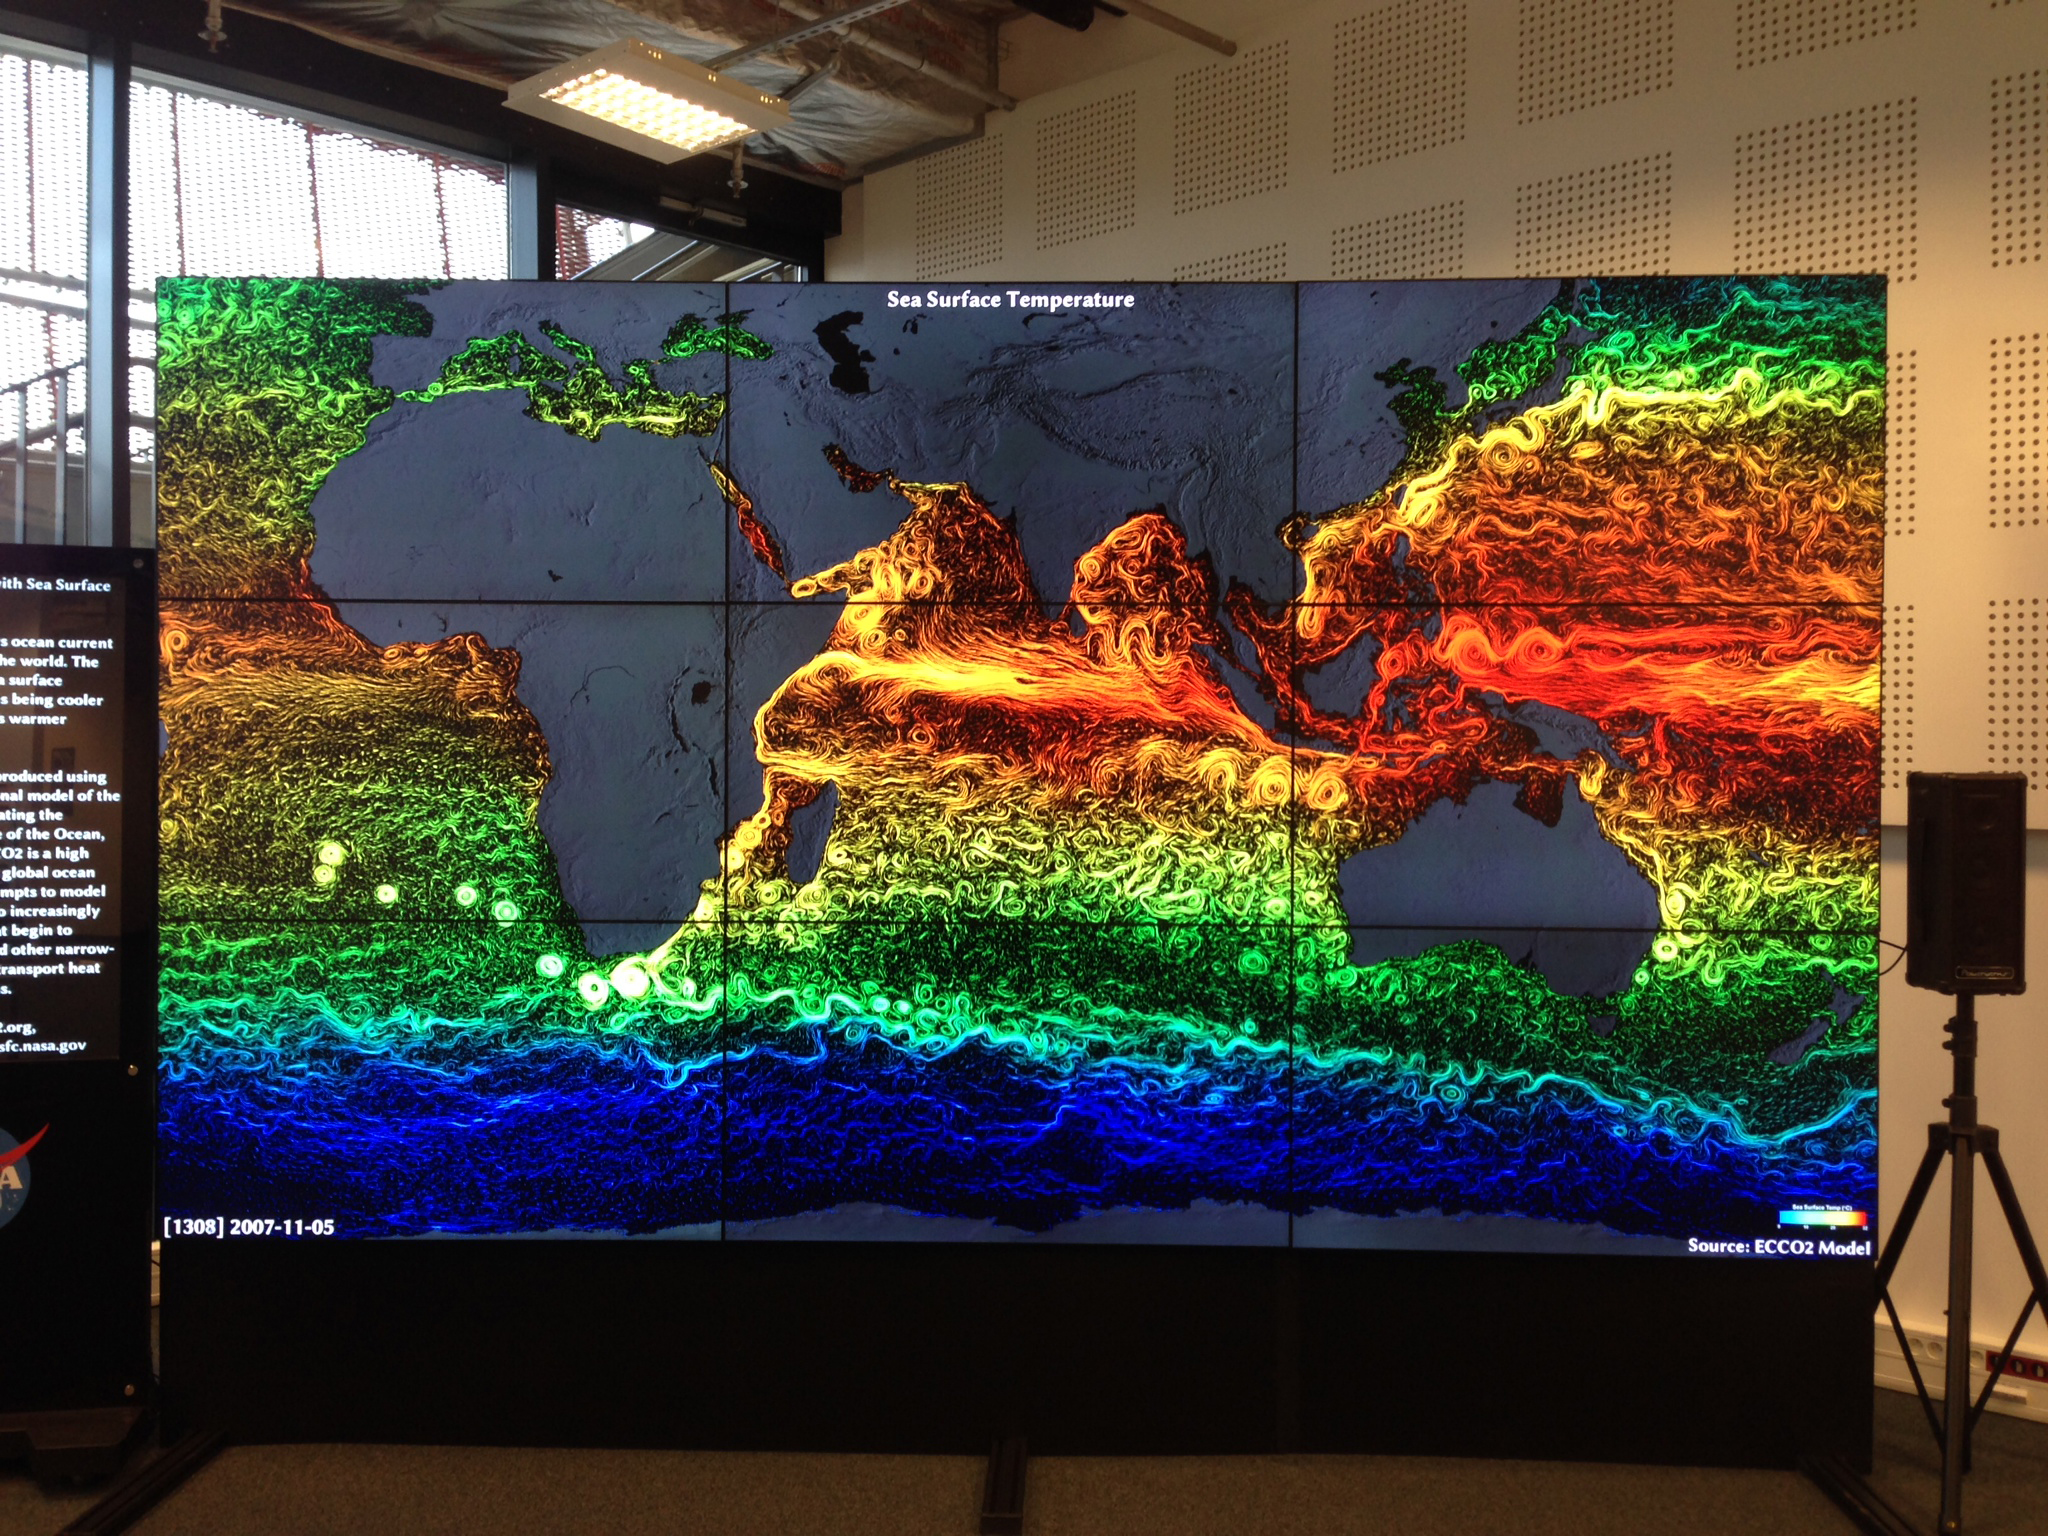
\includegraphics[width=\linewidth,height=91pt,keepaspectratio]{figures/large-display.jpg}\hfil}\vfil}
\smallskip{\scriptsize\sffamily Wall-scale display\par}
\end{minipage}\hfill
\begin{minipage}[t]{0.192\textwidth}\centering
{\small\sffamily\bfseries (c) VR}\par\smallskip
\vbox to 91pt{\vfil\hbox to \linewidth{\hfil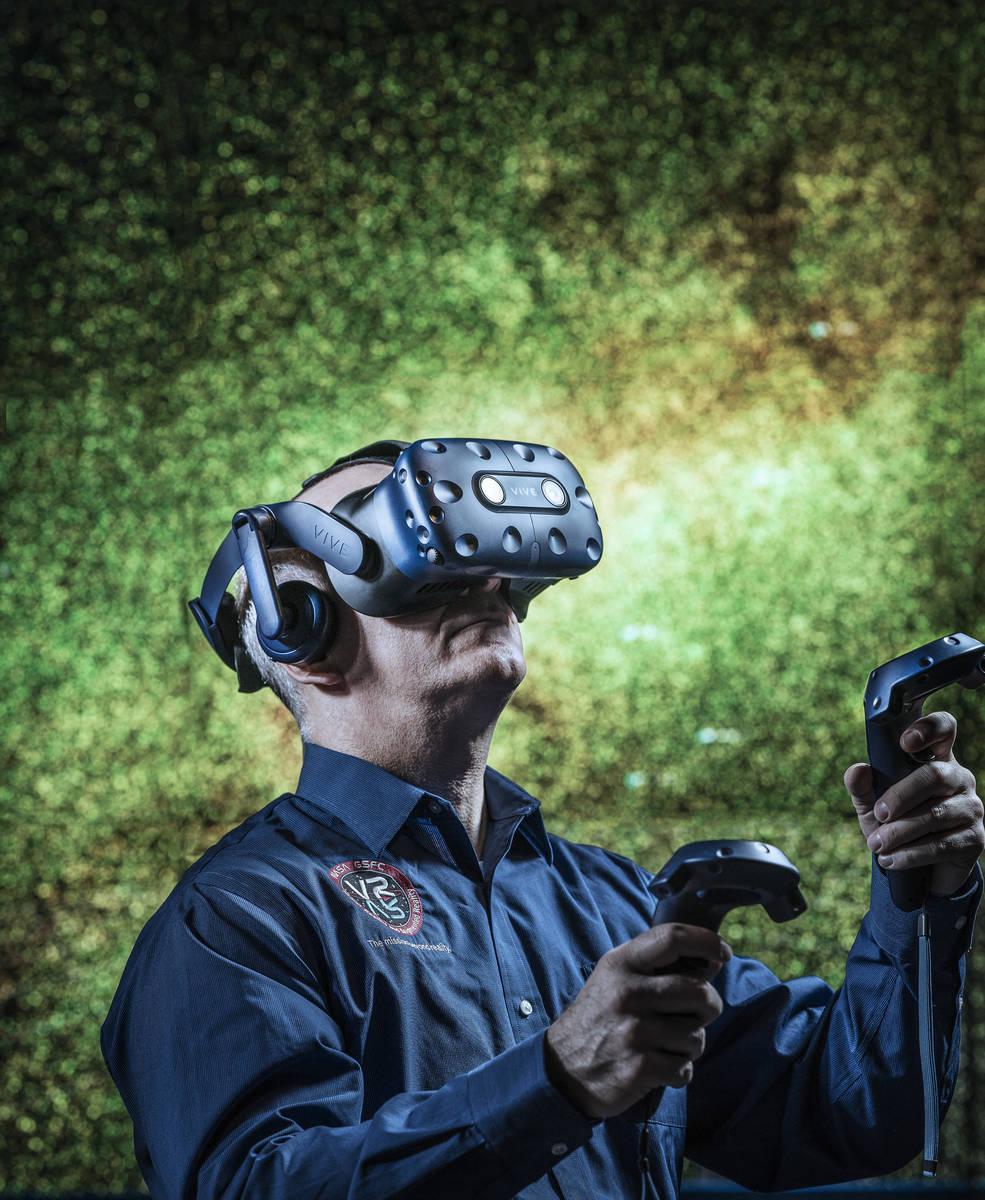
\includegraphics[width=\linewidth,height=91pt,keepaspectratio]{figures/vr.jpg}\hfil}\vfil}
\smallskip{\scriptsize\sffamily Head-mounted virtual scene\par}
\end{minipage}\hfill
\begin{minipage}[t]{0.192\textwidth}\centering
{\small\sffamily\bfseries (d) AR/MR}\par\smallskip
\vbox to 91pt{\vfil\hbox to \linewidth{\hfil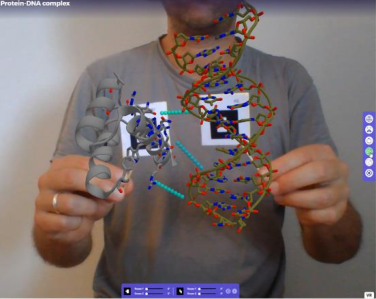
\includegraphics[width=\linewidth,height=91pt,keepaspectratio]{figures/system-examples/molecularweb_panel_e.pdf}\hfil}\vfil}
\smallskip{\scriptsize\sffamily Digital + physical context\par}
\end{minipage}\hfill
\begin{minipage}[t]{0.192\textwidth}\centering
{\small\sffamily\bfseries (e) CAVE}\par\smallskip
\vbox to 91pt{\vfil\hbox to \linewidth{\hfil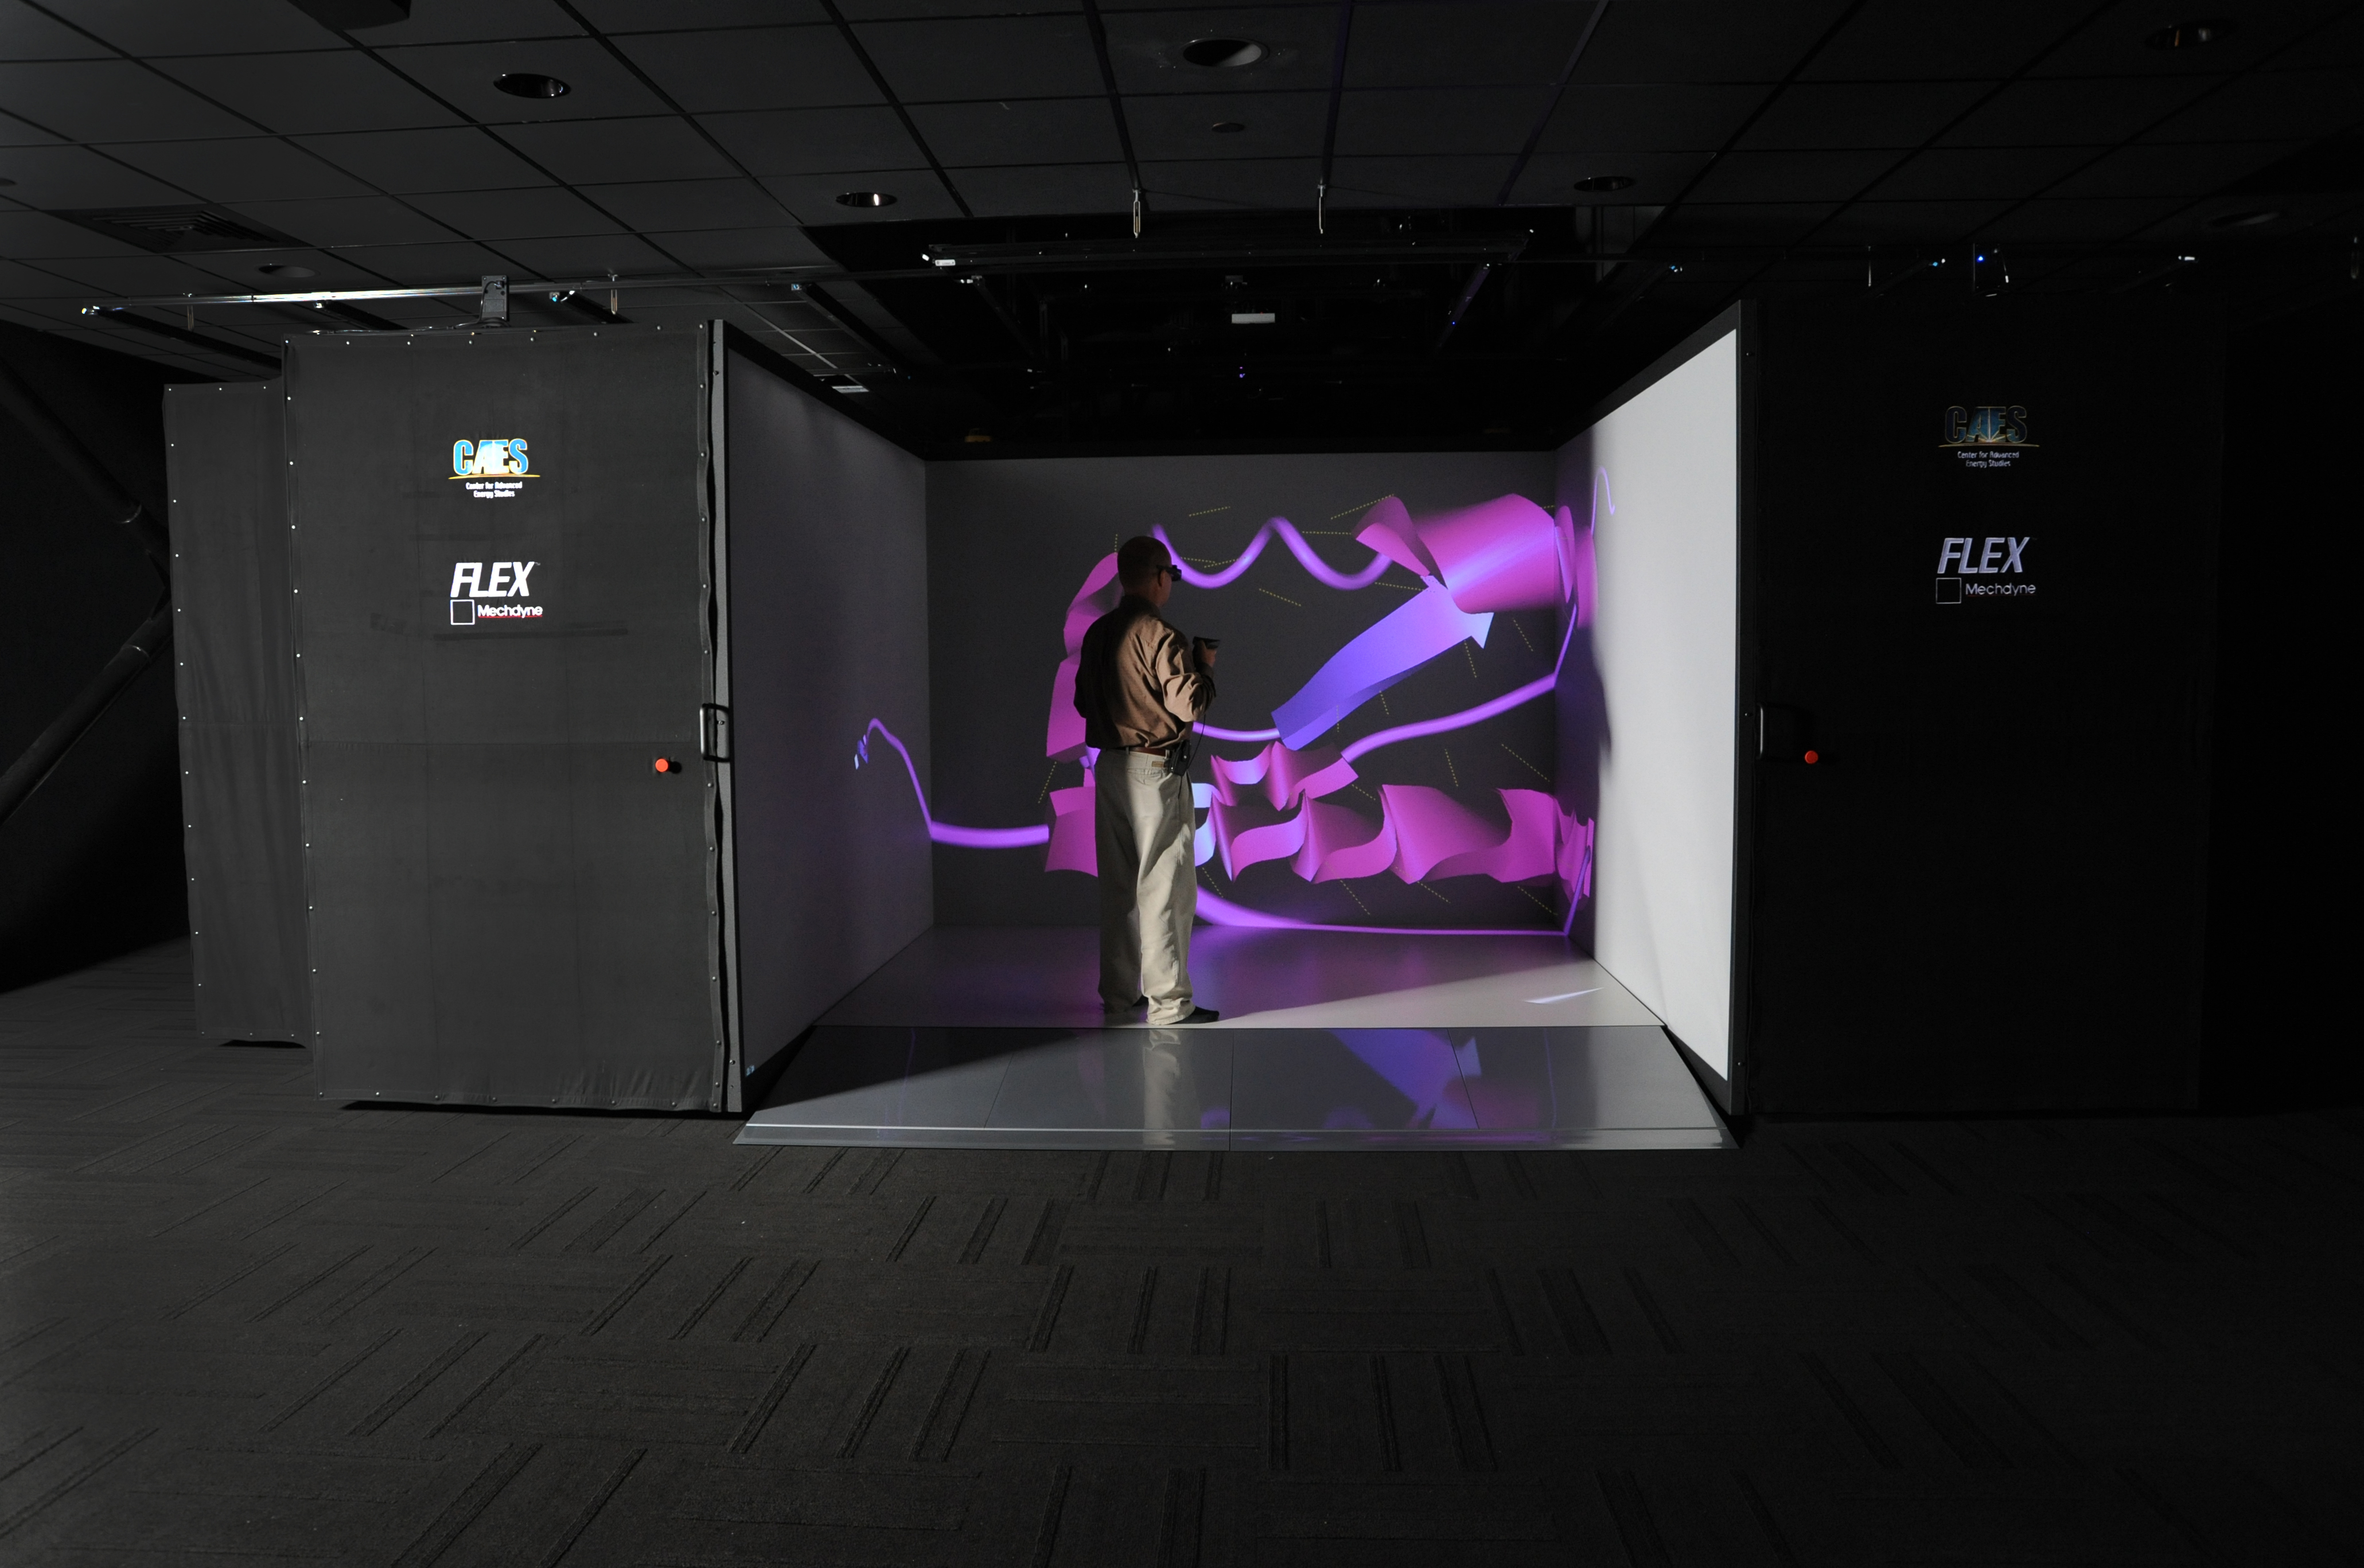
\includegraphics[width=\linewidth,height=91pt,keepaspectratio]{figures/cave.jpg}\hfil}\vfil}
\smallskip{\scriptsize\sffamily Surrounding projections\par}
\end{minipage}
\caption{Examples of the five visualization environments used in this review: (a) a desktop research workstation; (b) NASA's tiled Hyperwall; (c) a virtual-reality headset and controllers; (d) moleculARweb superimposing protein and DNA models on a camera view of handheld markers; and (e) a CAVE displaying a protein model. These images illustrate interaction environments, not assistance mechanisms or evidence of analytic benefit. Photographs (a--c) and (e) reproduced without additional cropping: (a) \href{https://commons.wikimedia.org/wiki/File:Scientist_working_with_personal_computer,_2013_(Dell_Precision_T3500_Workstation).jpeg}{Jennie Groom/IPAS (Commons derivative)}, (c) \href{https://commons.wikimedia.org/wiki/File:Exploring_the_Universe_in_Virtual_Reality.jpg}{NASA/Chris Gunn}, and (e) \href{https://commons.wikimedia.org/wiki/File:Cave_automatic_virtual_environment.jpg}{Idaho National Laboratory}, each \href{https://creativecommons.org/licenses/by/2.0/}{CC BY 2.0}; (b) \href{https://commons.wikimedia.org/wiki/File:NASA's_Hyperwall_Shows_the_Sea_Surface_Temperature_(10946045463).jpg}{U.S. Department of State}, public domain in the United States. Panel (d) cropped from Abriata~\cite{Abriata2025MolecularWebUniverse}, Fig.~1(E), \href{https://creativecommons.org/licenses/by/4.0/}{CC BY 4.0}.}
\label{fig:modality-environments}
\end{figure*}


\emph{Desktop/Planar} environments present analysis through conventional screen-based views, including two-dimensional diagrams and three-dimensional scenes rendered on a monitor. \emph{Large Display} environments provide an expanded display surface, such as a wall or tabletop, around which views and participants can be arranged. \emph{VR} environments present a virtual setting through a head-mounted display. \emph{AR/MR} environments combine digital information with a view of physical surroundings, with varying degrees of spatial registration and interaction between them. \emph{CAVE} environments use projections across multiple surrounding surfaces to present an immersive scene. We retain CAVE as a separate category because its shared physical space and projection-based presentation differ from head-mounted VR.

Display environment, input channel, and computational assistance describe different aspects of a system. A desktop application may accept speech or tracked gestures, while a VR application may use menus and explicit commands. A three-dimensional embedding displayed on a monitor remains a Desktop/Planar environment under these definitions. Similarly, a matrix displayed within a virtual workspace remains part of a VR environment. Modality is identified from the interaction environment; initiative and control are assessed from the analytical operations and decisions within it.


\subsection{Locus of Analytic Agency}
\label{subsection:locusofagency}

We use \emph{locus of analytic agency} to describe who takes the initiative and who controls decisions during visual analysis. This can change as a workflow proceeds. A scientist may define a question, ask a system to identify promising structures, revise its suggestions, and assess their biological meaning. Holter and El-Assady~\cite{HolterElAssady2024Agency} (§4.1) describe agency in terms of control over the analysis process and responsibility for decision-making. They also discuss how control can depend on the stage of interaction. Building on this perspective, we examine how scientists and computational systems share decisions within an analytic workflow.

Different parts of a task can involve different divisions of work. An analyst who requests a comparison may let the system select candidates and calculate differences while retaining control over the comparison criteria and interpretation. Monadjemi et al.~\cite{Monadjemi2026MixedInitiative} (Sections~5.1--5.2) examine how humans and artificial agents contribute to shared analytic tasks, including setting constraints, recommending actions, and contributing knowledge. For this review, we ask who proposes an operation, who chooses its scope and parameters, who performs it, and who assesses the result. We also ask whether the analyst can inspect, change, or undo what the system has done. These questions guide our comparison of workflows. Later references to analytic agency concern this operation-level account of proposal, scope, execution, and assessment, together with opportunities to inspect, change, or undo an action.

This example distinguishes between carrying out an operation, proposing the next step, and judging what a result means. A calculation may be fully automated even though the scientist has chosen its purpose, inputs, and parameters. A recommendation can influence the direction of analysis even when the scientist must approve it. Monadjemi et al.~\cite{Monadjemi2026MixedInitiative} (Section~5.1 of their review) observe that recommendations may indirectly shape analytic goals; they also emphasize that mixed initiative need not involve high levels of automation (their Section~5.4). In scientific analysis, a further question is whether the evidence supports the resulting interpretation. A system may suggest a biological explanation, but that suggestion still needs to be checked against the data and the assumptions behind the analysis. We therefore examine what opportunities analysts have to check results, consider alternatives, and correct earlier decisions. An approval button alone does not tell us whether those opportunities are available.


\subsection{Positioning Against Existing Reviews and Frameworks}
\label{subsection:priorreviews}

The preceding distinctions bring together several strands of visualization research. Biological network surveys examine how relationships are represented and explored. Immersive analytics reviews examine the environments in which this exploration takes place. Research on automation and human--AI collaboration examines how people and computational systems contribute to the work. These perspectives provide complementary foundations for studying assisted analysis in the life sciences.

Ehlers et al.~\cite{Ehlers2025} organize their survey of biological network visualization around the visualization pipeline, following the progression from data to visual structures and views through task-driven interaction. This connects biological data, representation, and analytic use. Our review builds on that connection by asking how computational assistance participates in decisions along the pipeline: which relationships are selected, how they are transformed, what receives attention, and how the resulting patterns are assessed.

Kraus et al.~\cite{Kraus2022ImmersiveAnalyticsSurvey} review immersive analytics using abstract three-dimensional visualizations, with a scope centered on stereoscopic environments. Their review provides a foundation for considering immersive approaches to relational data. Here, we examine assistance across immersive, desktop, and large-display environments, including workflows that use different representations or combine settings. The comparison concerns how an environment supports computational participation in the analysis.

Mixed-initiative and automation frameworks address the division of work more directly. The Domova and Vrotsou model~\cite{DomovaVrotsou2023Automation} describes types and levels of automation across stages of visual analysis. Holter and El-Assady~\cite{HolterElAssady2024Agency} distinguish agency, interaction, and adaptation within human–AI collaboration. Monadjemi et al.~\cite{Monadjemi2026MixedInitiative} examine human and artificial contributions to shared visual analytic tasks, together with levels of automation and evaluation practices. Our contribution is the application of these established agency concepts to relational and multiscale life-science analysis. We connect who proposes, scopes, performs, and assesses particular operations, and who can inspect or revise them, to the implemented mechanism, display environment, and evidence supporting a scientific interpretation. This domain-specific comparison links the Assistance $\times$ Visualization Modality framework to evaluation requirements for the five task groups.



Sections~\ref{sec:tasks}--\ref{sec:modality} apply these distinctions to selected system comparisons. Assistance--modality placements organize mechanisms and environments; the comparisons examine specific analytical actions within that space. Initiative and control can differ across actions within the same workflow. We therefore examine the division of work for each action, including the opportunities scientists have to inspect and revise its consequences, and relate it to the evaluation requirements discussed in Section~\ref{sec:evaluation}.


Figure~\ref{fig:assistance-modality-map} makes these distinctions concrete. It locates representative mechanisms within the two axes, while task symbols connect those placements to the purposes examined in Section~\ref{sec:tasks}. The planar examples include configured analysis, feedback-driven learning, and language-mediated execution.~\cite{AnchorRNASeqEZPZ,AnchorFacetto,AnchorPeCaX,AnchorMetis,AnchorFathomGPT,EvalKim2025} Echo, NUI-VR$^2$, ProteinSketch, DTBIA, the skin-lesion AR application, and iCAVE extend the comparison across display environments.~\cite{MapEcho,AnchorNUIVR,AnchorProteinSketch,MapDTBIA,MapSkinAR,MapICAVE} The expanded map includes 76 systems with 119 supported system--cell placements within a 381-system set selected for assessment. These counts describe assessed coverage, not the frequency of approaches in the provisionally coded candidate pool. Analytic agency is examined through their mechanisms rather than encoded as an additional ranking. Vitessce Link's Immersive--AR/MR placement is supported by embodied specification of geometric measurement in the report's Supplementary Note 1 (I5) and Supplementary Note 4.~\cite{ExpansionX015} The dashed cells reflect the targeted assessment described in Section~\ref{sec:methodology-assessment}; unresolved eligibility and unverified mechanism--environment relationships are retained separately from supported placements.

%%\begin{figure*}[t]
\centering
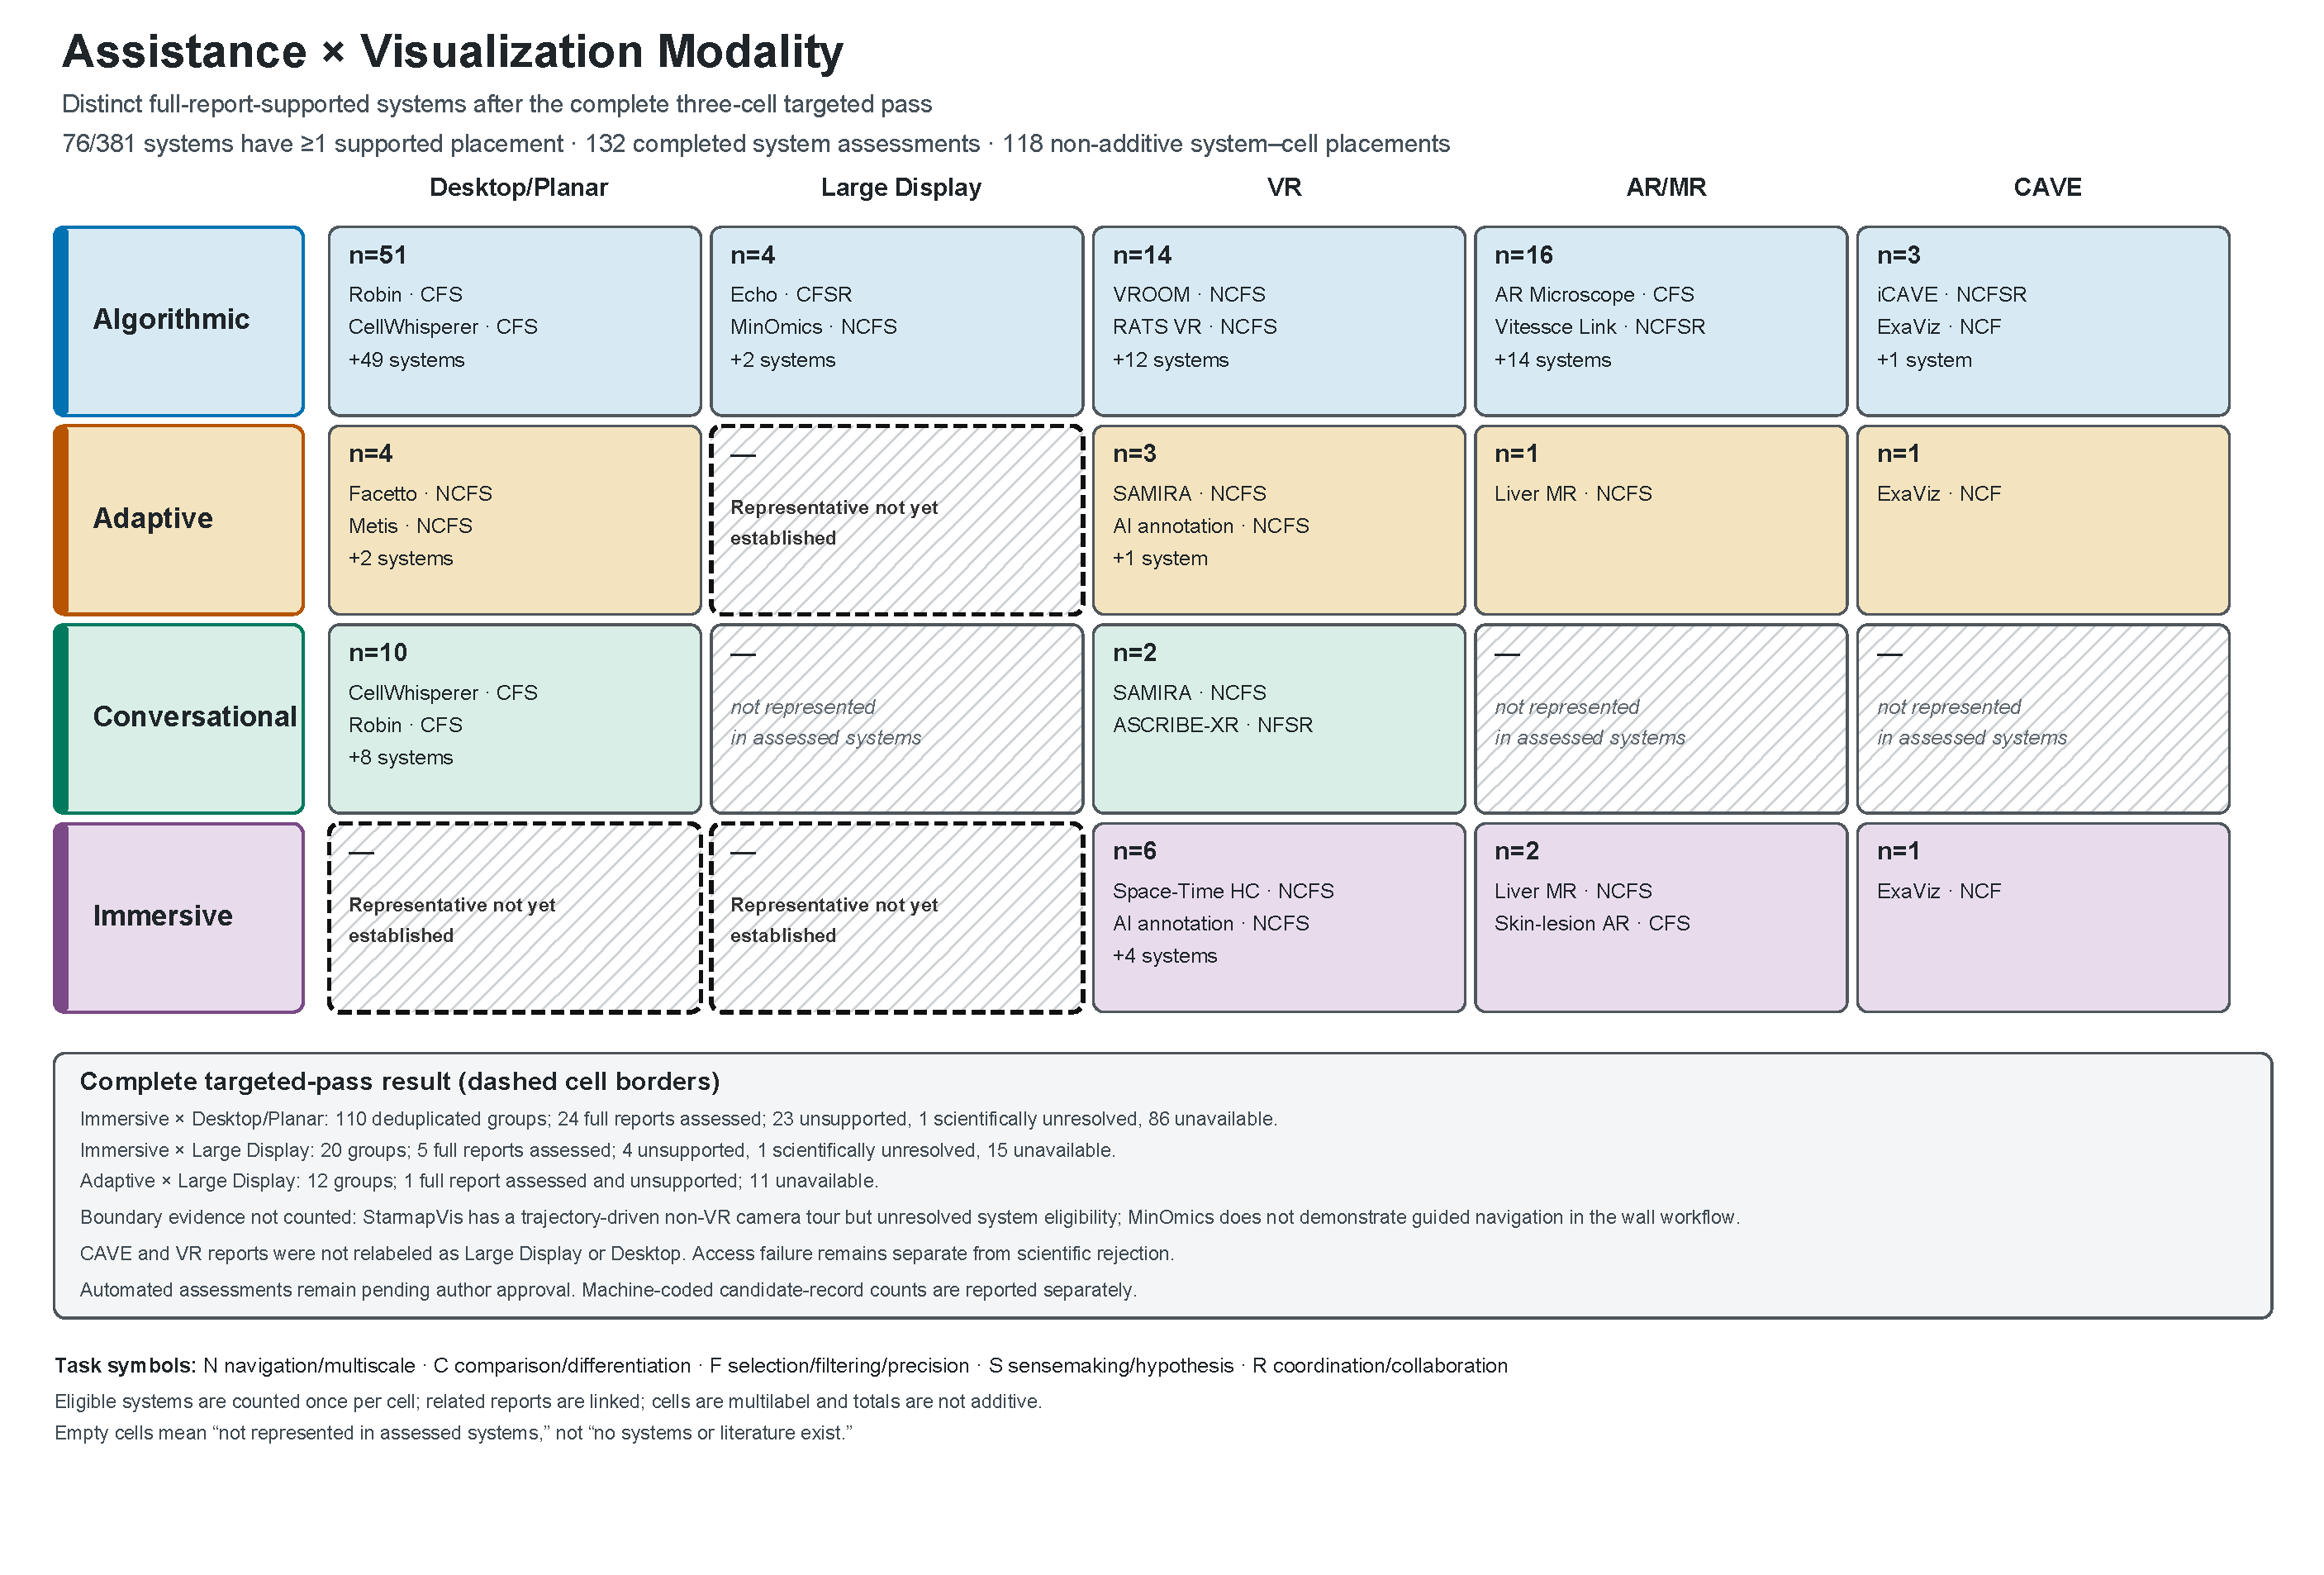
\includegraphics[width=\textwidth]{evidence/targeted-coverage/figure2_targeted_assistance_modality_map.pdf}
\caption{Assistance $\times$ Visualization Modality in the bounded assessment set: 381 systems considered, 132 completed system-level assessments, and 76 systems supporting 118 system--cell placements. Each $n$ counts distinct systems with evidence for that particular mechanism--environment relationship; counts are multilabel and non-additive. Names illustrate selected placements, and task letters follow the evidence matrix. Unfilled cells indicate that a representative has not yet been established, not absence from the literature. Contextual, inaccessible, and unresolved placements are not counted. These assessment counts are separate from machine-coded candidate co-occurrences and do not estimate literature prevalence.}
\label{fig:assistance-modality-map-old}
\end{figure*}

\begin{figure*}[t]
  \centering
  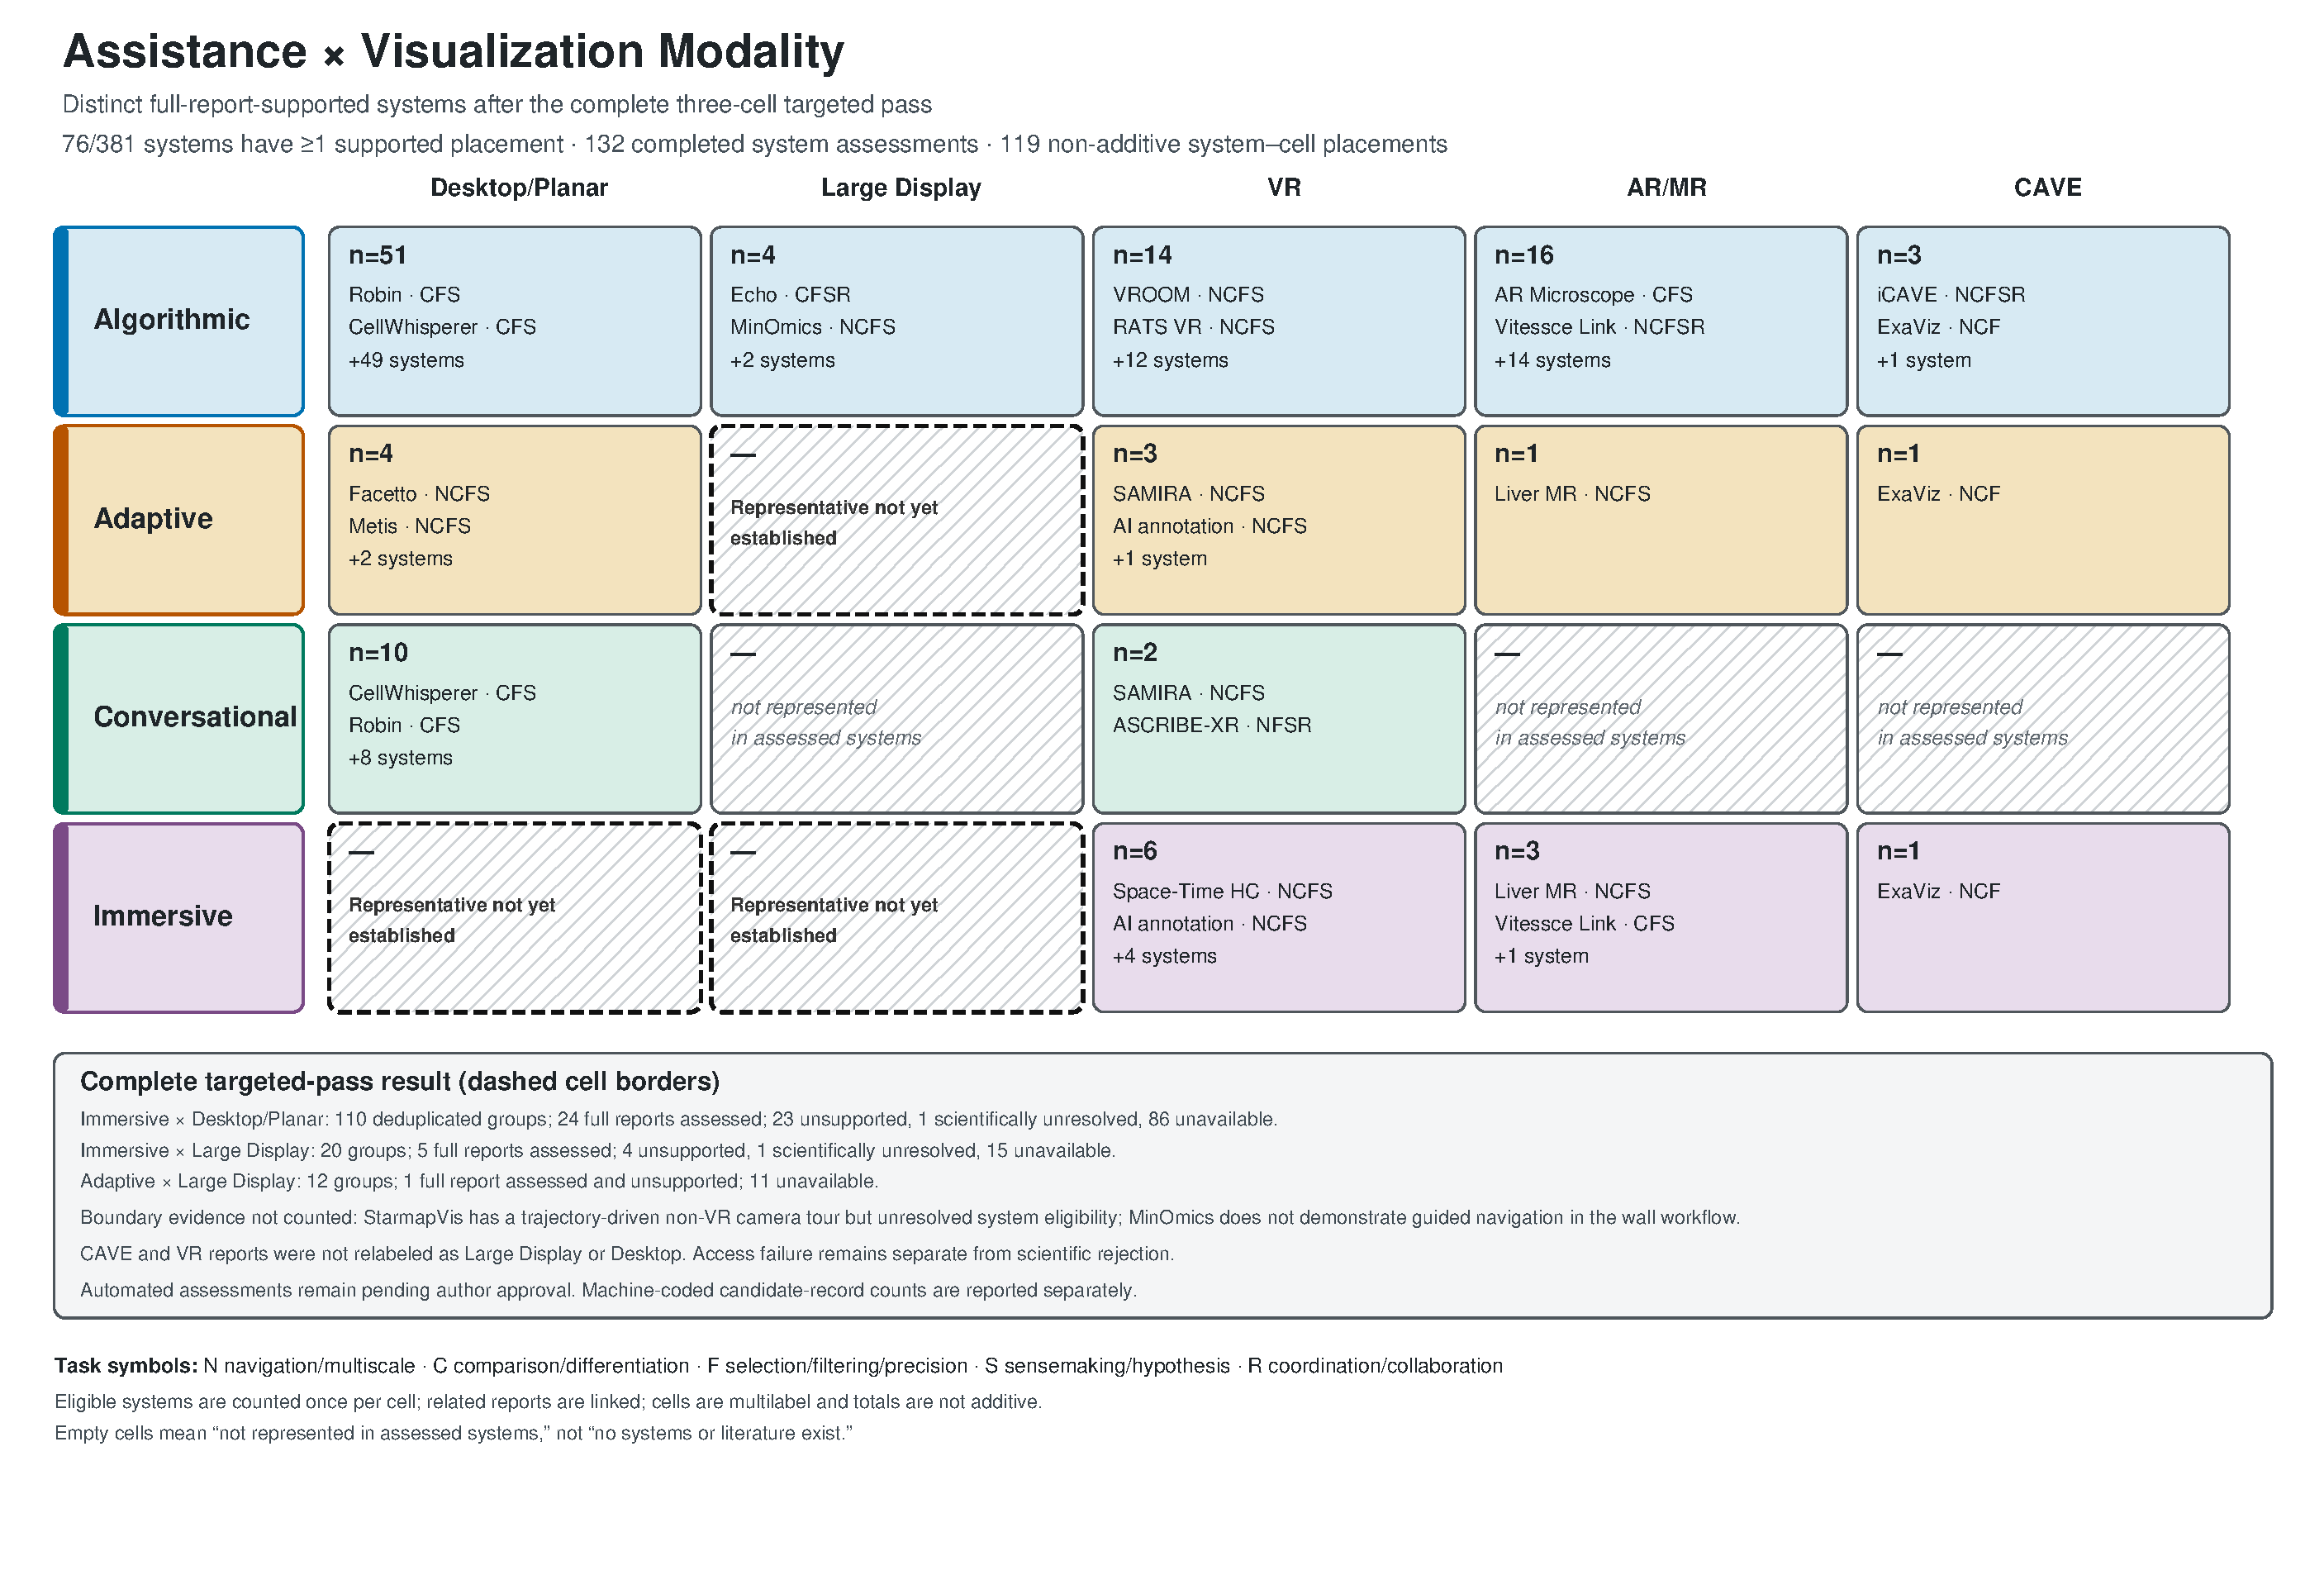
\includegraphics[width=\textwidth]{figures/figure3_assistance_modality_map.pdf}
  \caption{Assistance $\times$ Visualization Modality map of 76 systems with 119 supported system--cell placements, drawn from 132 completed assessments within a selected set of 381 systems. Each count represents a distinct eligible system with report-level evidence for the assistance--modality combination. Systems can occupy several cells, so counts are not additive. Dashed cells indicate that a representative was not established by the targeted assessment; empty cells indicate no representation in the assessed set, rather than absence from the literature. Task symbols denote navigation (N), selection/filtering (F), comparison (C), sensemaking (S), and collaboration (R). Candidate-record discovery counts are separate from supported placements. Section~\ref{sec:methodology-assessment} explains selection and targeted coverage; Section~\ref{subsection:priorreviews} explains the map's interpretation.}
  \label{fig:assistance-modality-map}
\end{figure*}

\section{Analytic Tasks and the Changing Locus of Agency}
\label{sec:tasks}

We compare systems by the analytical work scientists seek to accomplish and the computational contributions used to support it. For each task, we examine what computation performs, which decisions scientists supply or retain, and how they can inspect and revise the result. The Assistance $\times$ Visualization Modality framework organizes the mechanisms and environments involved; the locus of analytic agency identifies differences in initiative and control over particular actions. These comparisons connect system capabilities to the evaluation questions needed to assess their analytical benefits.

The five task categories introduced in Section~\ref{sec:foundations} describe related purposes rather than successive stages. Scientists revisit selections, comparisons, and explanations as questions develop. We therefore compare systems around consequential actions, reserving implementation detail for Section~\ref{sec:assistance} and environmental conditions for Section~\ref{sec:modality}. An interaction can support several tasks, but its presence does not establish that every task is supported equally well.

The task symbols in Figure~\ref{fig:assistance-modality-map} allow these purposes to be followed across assistance modes and environments; sharing a symbol does not imply equivalent task support or performance.

\subsection{Navigation and Multiscale Orientation}
\label{sec:tasks-navigation}

Navigation concerns locating relevant information while retaining enough context to understand its relationships. In life-science analysis, the problem includes movement between a local structure and its wider network, or between an observed specimen and a computed feature space. Panning and zooming change the visible region; computational organization also changes the structure through which the scientist navigates. The distinction matters because an accessible overview is already a selection of what to emphasize.

Compressed Adjacency Matrices organize regulatory networks so that motifs, paths, and neighborhoods can be inspected through highlighting, filtering, and selected views.~\cite{AnchorCompressedMatrices} Facetto connects tissue images with feature distributions, projections, and phenotype organization.~\cite{AnchorFacetto} The former makes network structure traversable through a computed representation; the latter supports inspection across spatial and derived descriptions of cells. These examples concern orientation among relationships and representations. They should not be recast as demonstrated autonomous navigation or guided scale changes without evidence of those mechanisms.

Agency lies partly in who chooses the next object of attention and partly in how the available overview was constructed. A scientist may control every movement while relying on computational abstractions to determine what is readily visible. Evaluation should consequently distinguish reaching a target from maintaining context, recognizing omitted structure, and returning to an earlier observation. A display may make traversal easier without improving those other outcomes. The modality comparison must identify which of these costs a change of environment actually addresses.

\subsection{Selection, Filtering, and Precision Interaction}
\label{sec:tasks-selection}

Selection establishes which entities or relationships an analysis concerns. Direct pointing specifies an object; filtering specifies conditions; assisted selection may infer membership from examples or translate a request into a set. These actions can produce similar-looking highlights while assigning different responsibility for the selected population. Precision therefore has both an interaction meaning, selecting the intended object, and an analytical meaning, forming a set appropriate to the question.

Facetto makes this distinction consequential when experts select image regions or feature groups and revise phenotype labels. Feedback can affect later classifier assignments beyond the cells directly inspected.~\cite{AnchorFacetto} In FathomGPT, a language request can instead determine the queried records through generated SQL.~\cite{AnchorFathomGPT} The scientist provides examples in one case and a description in the other; computation contributes to the resulting membership. Checking a selected set requires access to the relevant basis for membership, not merely confirmation that a selection action succeeded.

NUI-VR$^2$ illustrates a spatial counterpart: user-supplied seeds and parameters influence computed segmentation boundaries.~\cite{AnchorNUIVR} A precise gesture and an accurate segmentation are related but distinct accomplishments. Its technical segmentation measures assess the resulting boundary, not the full effort of choosing seeds, detecting errors, and correcting them. Across these mechanisms, the useful comparison is how scientists specify intent, inspect the selected result, and recover from unintended inclusion or omission. That comparison can then inform whether planar input, language, or spatial interaction suits the particular selection problem.

\subsection{Comparison and Differentiation}
\label{sec:tasks-comparison}

Comparison requires a reference: another observation, condition, model, source, or expected pattern. Computation can establish correspondence, derive differences, and organize cases for inspection, but those choices shape what a visible difference means. A salient contrast may reflect measurement, representation, or modeling choices, rather than a biological distinction. The analyst's responsibility therefore includes deciding which comparisons are meaningful and which alternative explanations remain plausible.

RetainVis and MediSyn locate this work at different evidential levels. RetainVis exposes risk predictions and feature contributions across patients and cohorts, with editing and retraining that can change inputs or model state.~\cite{AnchorRetainVis} MediSyn aligns biomedical assertions across datasets and makes provenance, coverage, and disagreement inspectable.~\cite{AnchorMediSyn} In the former, comparison can investigate how a computed inference responds to intervention; in the latter, it can investigate where sources support or contradict an interpretation. An input edit is not evidence of a real-world causal effect, just as agreement among displayed assertions is not by itself proof of their independence or correctness.

The distinction also changes the evaluation target: RetainVis's model behavior and MediSyn's evidence-selection performance are not interchangeable outcomes. Section~\ref{sec:evaluation-effectiveness} separates computational behavior from analytical and scientific benefit.

Comparison can also interrogate the representation itself. focusedMDS/distnet exposes discrepancies between projected and high-dimensional distances, while PathwayMatrix uses ordering, grouping, and lenses to inspect pathway relationships.~\cite{ExpandedE34,ExpandedE37} PAE Viewer links predicted alignment error with protein structure and cross-links, making model reliability an object of inspection rather than an implicit property of the display.~\cite{ExpandedE49} By contrast, CoCoNUT's sequence comparisons and Toxygates' clustering and enrichment organize evidence about genomic similarity and response patterns.~\cite{ExpandedE35,ExpandedE36} These mechanisms support different comparisons even when their interfaces share planar views.

\subsection{Sensemaking and Hypothesis Development}
\label{sec:tasks-sensemaking}

Sensemaking connects observations with possible explanations and questions for further investigation. Assistance may expose a pattern, suggest a candidate, or execute an analysis that tests part of an interpretation. The scientific work includes deciding what the result warrants and what further evidence is needed. A computationally generated possibility becomes useful through that relationship to an investigation, rather than through generation alone.

RNA-SeqEZPZ provides interactive outputs from a configured transcriptomics pipeline, while FathomGPT lets scientists formulate and refine requests that become queries and visual results.~\cite{AnchorRNASeqEZPZ,AnchorFathomGPT} Both support inquiry, but the route from question to computation differs. In the first, scientists configure an established sequence and interpret its output; in the second, they also inspect the translation of language into analytic operations. Neither route transfers responsibility for biological interpretation merely because execution is delegated.

Metis and ProteinSketch extend the task toward constructing candidates: feedback and spatial specifications shape which molecular possibilities are generated.~\cite{AnchorMetis,AnchorProteinSketch} Their mechanisms are compared in Sections~\ref{sec:assistance-adaptive} and~\ref{sec:assistance-immersive}. Here, the task consequence is that scientists must assess not only a candidate, but also the constraints and omissions that shaped the candidate space.

The agency consequence is a change in the space of possibilities presented to the scientist. Exposing why a candidate was generated, what constraints shaped it, and what alternatives were not considered can support critical interpretation. These are design implications of the workflows, not evidence that either system has demonstrated unbiased exploration. Section~\ref{sec:evaluation} considers how to assess those claims.

\subsection{Coordination and Collaborative Reasoning}
\label{sec:tasks-coordination}

Collaborative analysis requires more than making the same visualization available to several people. Participants must divide work, communicate interpretations, recognize changes, and determine which results or revisions can be accepted. Computational assistance can organize evidence for discussion or coordinate analytical actions. The distinction identifies whether a system primarily supports shared interpretation or the management of interdependent work.

PeCaX brings computed variant annotations and pathway relationships into a workflow intended for molecular-tumor-board inspection.~\cite{AnchorPeCaX} Its relevance to collective interpretation does not, by itself, establish a synchronous multiuser interface or automated management of disagreement. NeuroBlocks more explicitly connects segmentation and proofreading with task assignment, approval, provenance, and restoration.~\cite{AnchorNeuroBlocks} Here, coordination includes who acts on a result, how its status changes, and how prior work can be audited or recovered.

These functions distribute authority as well as effort. A proposed correction, an accepted segmentation, and a communicated interpretation need not carry the same status or belong to the same participant. Group-visible records of such distinctions can support common ground; a shared display alone cannot supply them. PeCaX's processing results and NeuroBlocks's qualitative collaborations establish different aspects of the implemented workflows. Claims about improved collective reasoning additionally require evidence about participants' understanding, reconciliation of interpretations, and use of the resulting decisions.

\subsection{Relationships Across Tasks}
\label{sec:tasks-synthesis}

Tasks connect across a workflow, so an intervention's consequences may emerge after the action it directly supports. Consider an illustrative analysis: a scientist locates a tissue region, selects a cell population, compares its characteristics, proposes an explanation, and discusses it with collaborators. If assistance changes the selection, it also changes the basis of the comparison and the evidence supporting the explanation. This sequence is an analytical illustration, not a claim that one selected system implements every step.

Table~\ref{tab:task-agency-synthesis} summarizes the resulting comparison questions. For each task, the comparison identifies the computational contribution, the decisions scientists make or delegate, and the opportunities to inspect and revise results. These differences connect the mechanisms examined next to specific evaluation requirements: preserving context, forming appropriate selections, establishing meaningful comparisons, assessing interpretations, and coordinating shared decisions.

% Requires booktabs and tabularx. Questions synthesize the discussion, not measured outcomes.
\begin{table*}[t]
\centering
\caption{Task-centered questions for comparing assistance mechanisms. The final column identifies evaluation questions; it does not claim that every cited system has evaluated them.}
\label{tab:task-agency-synthesis}
\small
\setlength{\tabcolsep}{4pt}
\renewcommand{\arraystretch}{1.15}
\begin{tabularx}{\textwidth}{@{}>{\raggedright\arraybackslash}p{.15\textwidth}>{\raggedright\arraybackslash}X >{\raggedright\arraybackslash}X >{\raggedright\arraybackslash}X@{}}
\toprule
Task & Computational participation & Consequential human choice & Evaluation question \\
\midrule
Navigation and orientation & Organize structure; connect spatial and derived views. & Choose attention and interpret the context retained or omitted. & Can analysts locate relevant structure, retain context, and return to prior observations? \\
Selection and precision & Infer membership, translate set descriptions, or compute boundaries from seeds. & Specify intent and correct inclusion or omission. & Does the result match the analytical question, and how difficult is correction? \\
Comparison and differentiation & Align evidence or expose differences in predictions and contributions. & Choose reference conditions and interpret the source of a difference. & Can analysts distinguish source disagreement, model behavior, and biological variation? \\
Sensemaking and hypothesis development & Execute inquiries or generate candidates under feedback and constraints. & Formulate questions, inspect assumptions, and determine what warrants further testing. & Are interpretations traceable, alternatives inspectable, and claims supported by appropriate evidence? \\
Coordination and collaborative reasoning & Organize shared evidence or track assignments, approvals, and revisions. & Divide work, authorize changes, and reconcile interpretations. & Do participants understand the status, provenance, and consequences of one another's actions? \\
\bottomrule
\end{tabularx}
\end{table*}


\section{Computational Assistance Across Analytic Workflows}
\label{sec:assistance}

Computational assistance changes both the objects available for analysis and the actions through which scientists investigate them. A computed layout makes relationships inspectable; a classifier propagates labels beyond the examples an expert has examined; a language interface translates a question into operations. The four assistance modes introduced in Section~\ref{sec:foundations} distinguish these contributions without assigning each system to a single category. We compare mechanisms by their inputs, computational behavior, outputs, and opportunities for human intervention. Tasks provide the purpose of that intervention, while the locus of analytic agency explains which decisions the scientist retains, supplies indirectly, or delegates.

Figure~\ref{fig:assistance-modality-map} maps representative systems across assistance modes and visualization environments. A system may occupy several cells when it combines multiple forms of assistance or supports multiple environments.

\subsection{Algorithmic Assistance: Transforming the Analytic Substrate}
\label{sec:assistance-algorithmic}

Algorithmic assistance establishes structures on which subsequent interpretation is based. Clustering and dimensionality reduction organize similarities; layout and aggregation make relationships tractable; annotation and ranking connect observations to candidate explanations. These transformations make selected properties easier to inspect while placing others outside the immediate view. Their analytical consequences therefore depend on how scientists choose inputs, inspect results, and relate computed structure to the underlying evidence. Dimensionality reduction illustrates this distinction. Espadoto et al. survey projection techniques using criteria including preservation of data structure, scalability, and robustness.~\cite{espadoto2021quantitative} These criteria help compare the computational transformation; evidence that a projection supports a particular biological interpretation must be assessed separately.

RNA-SeqEZPZ integrates quality control, alignment, counting, differential-expression analysis, and pathway analysis behind a Shiny interface. Scientists supply files and parameters, initiate the pipeline, and explore outputs through interactive views. The mechanism delegates execution of a configured sequence while leaving its purpose and interpretation with the scientist.~\cite{AnchorRNASeqEZPZ} PeCaX connects somatic-variant annotation and pathway-network construction to filtering, inspection, and annotation for molecular-tumor-board work.~\cite{AnchorPeCaX} Here, assistance makes relationships among variants, pathways, and treatment evidence available for consideration; it does not itself establish which interpretation should guide a clinical decision.

\begin{figure*}[t]
\centering
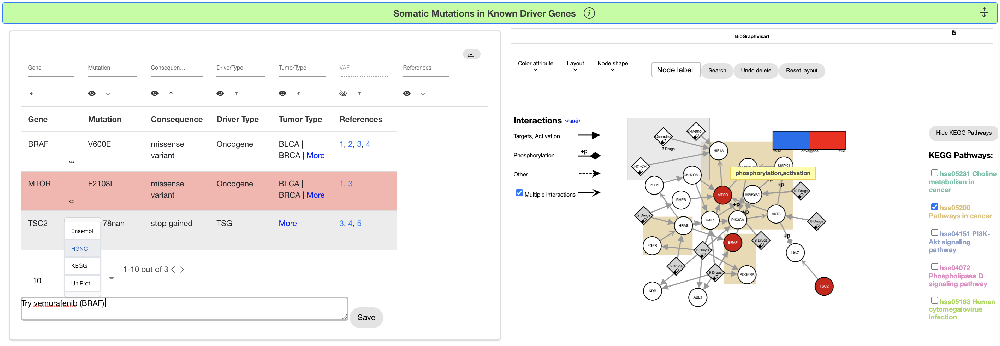
\includegraphics[width=\textwidth]{figures/system-examples/pecax_variant_network.pdf}
\caption{PeCaX connects annotated patient variants with gene--drug network context. The table summarizes somatic mutations in known driver genes, including predicted consequences, driver types, and reference sources; the associated network places affected genes alongside interacting genes and drugs, with controls for inspecting pathway context. Algorithmic annotation and network construction provide evidence that scientists can inspect when interpreting molecular findings. Cropped from Fig.~2 (upper table--network pair) in Additional file~1 of Figaschewski et al.~\cite{AnchorPeCaX}. \copyright{} The Author(s) 2023, licensed under CC BY 4.0 (\protect\url{https://creativecommons.org/licenses/by/4.0/}); cropping only.}
\label{fig:pecax-variant-network}
\end{figure*}


Representation-oriented systems expose a different point of intervention. Compressed Adjacency Matrices combine computational organization of gene regulatory networks with analyst-controlled rearrangement, highlighting, and filtering.~\cite{AnchorCompressedMatrices} Flud combines crowd-worker node placement with computational scores, clues, and simulated annealing.~\cite{bharadwaj2022flud} The comparison concerns how representational changes are distributed among analyst interaction, crowd work, and automated search. Flud’s layout and task results support its optimization strategy; an effect on biological discovery remains to be evaluated. Across these systems, the relevant question is what the transformation enables scientists to examine and how its assumptions remain available for scrutiny.

The same execution pattern appears in iGEAK, BioNetApp, OncoProExp, and SeqPlots: normalization, statistical comparison, clustering, aggregation, or pathway analysis remains connected to interactive inspection.~\cite{ExpandedE38,ExpandedE39,ExpandedE47,ExpandedE44} VIADS adds hierarchical aggregation and threshold-revisable summaries, while LIM Tracker couples automated tracking to manual correction and rerunning.~\cite{ExpandedE40,ExpandedE32} Virtual embolization instead lets analysts compare simulated occlusion alternatives on desktop and in VR.~\cite{ExpandedE30} These are distinct analytical substrates, not interchangeable demonstrations of autonomy.


\subsection{Adaptive Assistance: Responding to Analysis State}
\label{sec:assistance-adaptive}

Adaptive assistance depends on a relationship between an observed signal and a subsequent computational intervention. The signal may concern user feedback, developing task context, or data characteristics; the intervention may revise a model, prioritize candidates, or change guidance. Adaptation need not involve learned personalization, but it must be distinguished from simply exposing adjustable parameters. The useful comparison identifies what changes, why it changes, and how the scientist can influence that change.

Four questions make an adaptive mechanism explicit: what signal is observed, how it is used directly or interpreted as analytic context, what computational intervention changes in response, and what controls are available to the scientist. Signals may include explicit feedback, interaction history, task context, or data uncertainty; inferred goals and persistent user models are not required. Inspection, rejection, and reversal should be described as implemented capabilities where documented, and otherwise as design requirements. This account distinguishes what the system observes from what it assumes. Dwell time, for example, could indicate interest, confusion, or interruption; recording it does not establish that any one interpretation is correct.

Algorithmic processing and adaptation can consequently be coupled: a transformation produces candidate structures, while feedback or contextual information influences subsequent computation or presentation. The distinction does not depend on who initiates execution. Scientists may request adaptive guidance, and a fixed algorithmic pipeline may execute automatically. Nor is adaptation necessarily persistent learning: a context-dependent intervention and a model updated from feedback require different descriptions.

Facetto provides a concrete feedback loop. Experts inspect multiplex images and coordinated feature views, select regions and features, examine clusters, and revise phenotype labels. Those labels feed a classifier whose subsequent assignments change.~\cite{AnchorFacetto} The computational contribution is Algorithmic, while its response to expert labeling supports an Adaptive interpretation of that mechanism. Scientists supply examples that affect classification beyond the inspected cells. This makes checking later assignments consequential: a correction can alter the analysis more broadly than a local annotation. The implemented loop should also be distinguished from the report's proposed active-learning extension.

% Requires graphicx. Permission status: unconfirmed; see README.
\begin{figure*}[t]
  \centering
  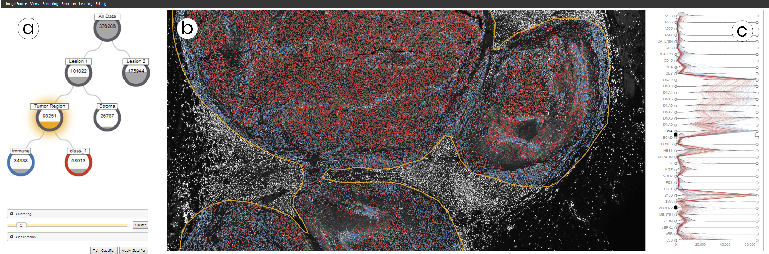
\includegraphics[width=\textwidth]{figures/system-examples/facetto_fig1_abc.pdf}
  \caption{Facetto links tissue inspection to expert-guided phenotype analysis. The phenotype tree (a) records analytical subsets, the tissue view (b) displays clustering and classification results in their spatial context, and the ridgeplot (c) supports feature inspection and filtering. These coordinated views let scientists inspect computational groupings and choose the cells and features used in subsequent analysis. Selected panels from Krueger et al.~\cite{AnchorFacetto}, Fig.~1(a--c); cropped from the original.}
  \label{fig:facetto-interface}
\end{figure*}


Metis places feedback at another point in analysis. Medicinal chemists evaluate generated molecules and identify favorable or unfavorable substructures. ~\cite{AnchorMetis} The system can fit a reward model to overall preferences or construct a reward function from supported feedback for integration into a configured REINVENT generation loop. The chemist supplies evaluations and initiates another run; some recorded feedback is not incorporated into generation. Compared with Facetto’s phenotype assignments, the affected objects are generated molecular candidates. The scientist influences which possibilities are produced or favored, rather than only interpreting an existing result.

% Requires graphicx. Permission status: unconfirmed; see README.
\begin{figure}[t]
  \centering
  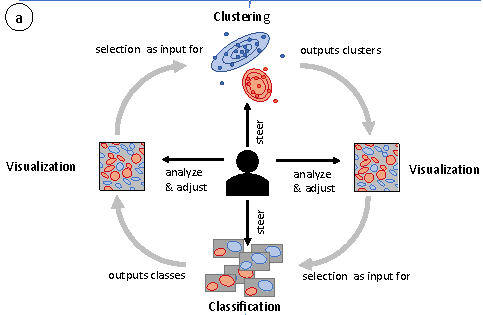
\includegraphics[width=\linewidth]{figures/system-examples/facetto_fig8a_loop.pdf}
  \caption{Facetto couples clustering and classification through an expert-guided analysis loop. Scientists inspect and adjust the visualized results, then select subsets that become inputs to the next computational step. The paper describes using labeled cells to train a classifier and clustering classification results to investigate further subgroups, connecting Algorithmic organization with Adaptive learning from expert input. Source: Krueger et al.~\cite{AnchorFacetto}, Fig.~8(a); cropped from the original.}
  \label{fig:facetto-learning-loop}
\end{figure}


Context-conditioned assistance does not need to learn a persistent user model. ExaViz computes viewpoints and paths from molecular geometry and a selected target, illustrating system-selected guidance rather than merely applying an entered camera position.~\cite{MapExaViz} SAMIRA conditions retrieved references and guidance on the current patient slice and spoken request; point-prompt segmentation corrections alone are not the basis for its Adaptive placement.~\cite{MapSAMIRA} The patient-health dashboard automatically selects visual modules from task and data characteristics, a narrower form of data-conditioned adaptive presentation rather than learned clinician personalization.~\cite{MapDashboard} These interpretations concern implemented selection of assistance; replay alone, fixed opacity weighting, and proposed future personalization do not establish the same contribution.

Facetto and Metis connect algorithmic processing with adaptation through analyst feedback. Facetto illustrates expert-directed analysis through guided cases, while Metis implements a feedback mechanism without reporting a participant outcome study. Their benefits therefore warrant evaluation at the task level: do revised outputs better serve the analyst’s goals, and can the analyst correct an inappropriate adjustment? Such evaluation should distinguish temporary concerns from lasting preferences and examine whether repeated prioritization limits exploration.

The feedback loop also changes the meaning of later signals. A recommendation can influence the next selection, which may then be treated as evidence of an enduring preference. Evaluating the inferred state independently of that influence is therefore important. The task determines what is at stake: a suggested region affects navigation, a propagated label changes a selection, and prioritized comparisons influence which explanations receive attention. Errors cannot be ranked by task name alone; a seemingly local selection error can propagate into subsequent comparisons and conclusions. Section~\ref{sec:evaluation} examines these consequences through intent accuracy, exploration breadth, appropriate reliance, and recovery rather than treating adaptation as a single performance score.

Further examples delimit responsive intervention. In interactive VR annotation, corrective positive and negative clicks trigger revised whole-volume segmentation.~\cite{ExpandedE24} Liver MR navigation uses newly acquired surface evidence to correct deformation of the preoperative model.~\cite{ExpandedE15} ASCRIBE-XR resolves underspecified segmentation, resolution, and meshing choices within a language-driven workflow; its Adaptive interpretation is limited to this context-conditioned selection, not learned personalization.~\cite{ExpandedE28} Fixed-threshold QC alerts and explicitly weighted aneurysm retrieval remain Algorithmic here.~\cite{ExpandedE48,ExpandedE46}

\subsection{Conversational Assistance and Agentic Orchestration}
\label{sec:assistance-conversational}

Conversational assistance changes the way analytic intent enters a computational workflow. A literal spoken command may duplicate a button, whereas a request to compare observations can require resolving entities, selecting data, constructing operations, and choosing a representation. The latter transfers some operational decisions to the system. Its scope depends on the implemented workflow: language input does not by itself establish autonomous planning, and a fluent explanation does not demonstrate correct execution.

FathomGPT connects natural-language questions about ocean data to scientific-name resolution, SQL generation and execution, and visual or image results. Conversation history supports refinement, while inspectable SQL exposes an intermediate representation of the requested operation.~\cite{AnchorFathomGPT} The scientist specifies a question and assesses the response; computation supplies steps that would otherwise require explicit query construction. This combines Conversational assistance with Algorithmic operations. It also illustrates bounded orchestration: the consequential delegation lies in translating a request into an executable sequence, without implying unrestricted system authority over scientific interpretation.

% Requires graphicx; uses the existing AnchorFathomGPT bibliography entry.
% Place fathomgpt_observer_map.png in figures/.
% Publication reuse permission remains unconfirmed; see README.md.
\begin{figure}[t]
  \centering
  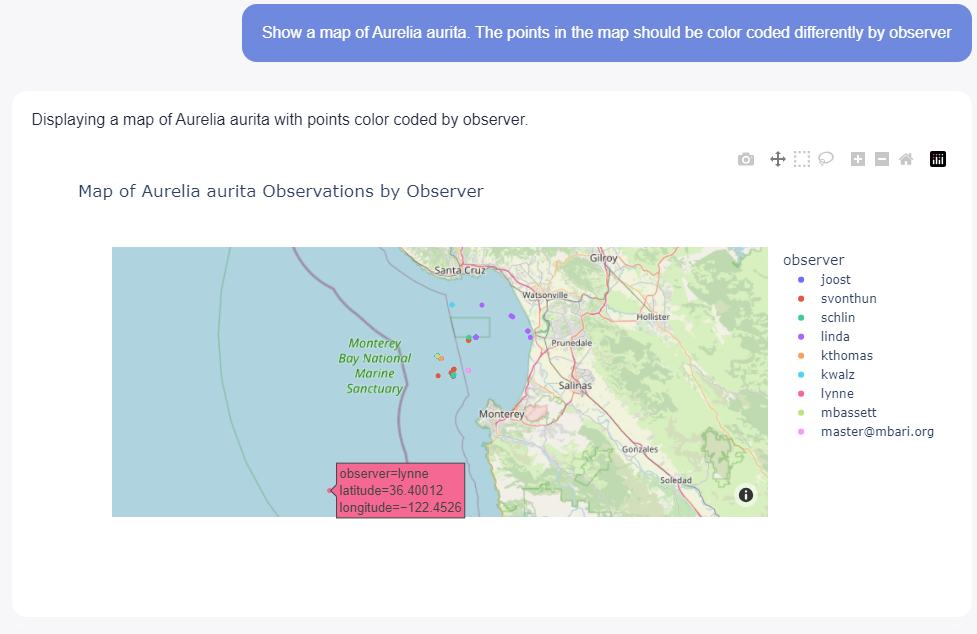
\includegraphics[width=\linewidth]{figures/system-examples/fathomgpt_observer_map.png}
  \caption{FathomGPT translates a natural-language request into an interactive map of \textit{Aurelia aurita} observations, with points colored by observer. The scientist specifies the species and grouping, while the system constructs the visualization; hovering reveals the observer and coordinates of an individual record. This connects Conversational assistance to spatial comparison and inspection of observation metadata on a Desktop/Planar display. Source: Khanal et al.~\cite{AnchorFathomGPT}, Fig.~12. Copyright 2024 held by the owner/author(s).}
  \label{fig:fathomgpt-observer-map}
\end{figure}


PhenoFlow provides a clinical counterpart: natural-language cohort requests are translated into data-wrangling code, accompanied by explanations and field-level views that neurologists can inspect.~\cite{EvalKim2025} Its model receives dataset metadata, including field names and coding information, rather than raw patient records. This bounds the translation mechanism; it does not remove the need to check whether the available fields support the intended cohort. FathomGPT and PhenoFlow thus make intermediate operations available for inspection while leaving scientific interpretation to the analyst.

General visual analytics examples expose further distinctions. LightVA separates planning, execution, and coordination, with on-demand task decomposition and opportunities to modify task flow.~\cite{LightVA} CausalChat represents proposed causal relationships and distinguishes LLM-suggested links that are not confirmed by data.~\cite{CausalChat} ProactiveVA instead uses interaction history and notes to infer possible needs and offer assistance.~\cite{EvalZhao2025} These illustrate workflow planning, hypothesis proposal, and context-dependent initiative, respectively; they are not interchangeable evidence of autonomous scientific reasoning. Their role here is contextual comparison, not automatic inclusion in the life-science corpus. A proposed causal link remains a hypothesis, and a plausible plan still requires examination of its operations and evidence.

Robin supports language-mediated comparison of genomic loop-caller outputs.~\cite{ExpansionX018} Users upload results generated by external loop-calling tools and inspect them through HiGlass, an integrated viewer for genomic contact maps. This separation makes the provenance boundary consequential: an explanation of uploaded results should remain distinguishable from execution of the analysis that produced them. A conversational interface does not erase that division of responsibility or establish adaptive intervention.

The contrast with Metis clarifies what interaction changes. A FathomGPT follow-up can revise a query or presentation; Metis feedback can alter the scoring or learning process that shapes later molecular candidates. Both accept high-level human guidance, but neither conversational continuity nor feedback collection alone establishes a persistent, accurate model of a scientist's goals. Inspection must address the relevant transformation: which data and operations a request selected, or how feedback affected subsequent outputs. Evaluation consequently needs to test whether a generated query represents the intended question and, for feedback-driven generation, whether candidate changes reflect the supplied feedback and remain open to correction.

FathomGPT's prompt-level evaluation supports successful interpretation and execution within its tested setting. Scientific conclusions drawn from a generated view additionally require examination of the data and assumptions behind the analysis. Analysts need to distinguish an account of an operation from its inputs, executed transformations, and results, using the provenance and control mechanisms discussed in Section~\ref{sec:evaluation}. The benefit of expressing intent in language must be considered alongside the work of verifying how that intent was operationalized.

\subsection{Immersive Assistance: Computational Use of Spatial Context}
\label{sec:assistance-immersive}

Immersive assistance uses spatial or embodied context, such as gaze, gesture, viewpoint, or body position, to guide computational support for an analytical task. The system interprets these signals to select, constrain, or adjust an operation: a spatial sketch, for example, can specify constraints that guide the generation of candidate molecular structures.

NUI-VR$^2$ couples VR gesture and voice interaction to segmentation and inspection of medical volumes. Seeds and parameters enter routines that compute probability maps and use feature selection; the resulting boundaries and volume views can then be examined.~\cite{AnchorNUIVR} The substantive assistance lies in the segmentation computation. Its spatial interface establishes VR use, but does not on its own demonstrate context-sensitive guidance, preference learning, or a separate Immersive assistance mechanism. Reported segmentation comparisons assess output behavior rather than establishing a general advantage for embodied interaction.

ProteinSketch provides a more direct connection between spatial expression and computational assistance. Users sketch secondary structures and volumes, providing spatial constraints for structure generation, sequence design, prediction, and filtering. ~\cite{AnchorProteinSketch} Spatial specification helps define a design space within which algorithms generate candidates. This coupling supports an Immersive interpretation alongside Algorithmic assistance: spatial input contributes analytically through its translation into computational constraints. The scientist specifies and interprets structures, while the pipeline supplies candidates that meet its implemented objectives. The preprint's computational and laboratory results support design feasibility; they do not isolate improved designer performance attributable to VR. Section~\ref{sec:modality} considers these environmental conditions separately from the mechanisms they host.

% Requires graphicx. Keep these PNGs alongside the manuscript, or adjust paths.
% Existing bibliography key: AnchorProteinSketch.
% DRAFT: confirm crop/publication reuse permission before submission.
\begin{figure*}[t]
  \centering
  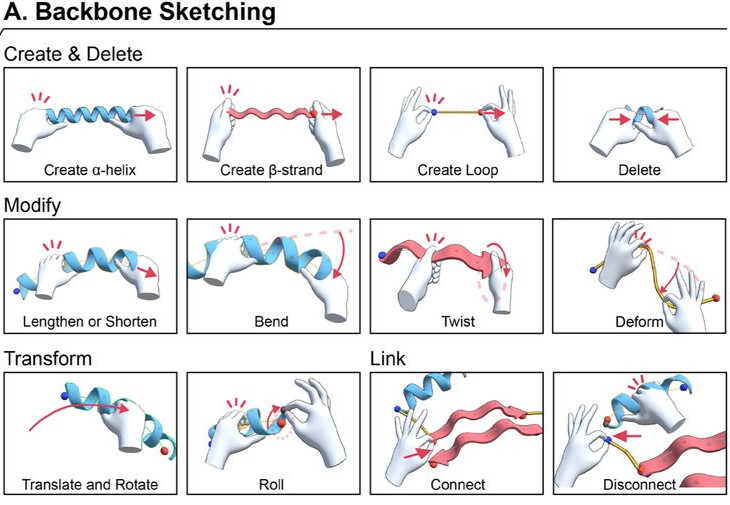
\includegraphics[width=0.64\textwidth]{figures/system-examples/proteinsketch_backbone_crop.png}\\[5pt]
  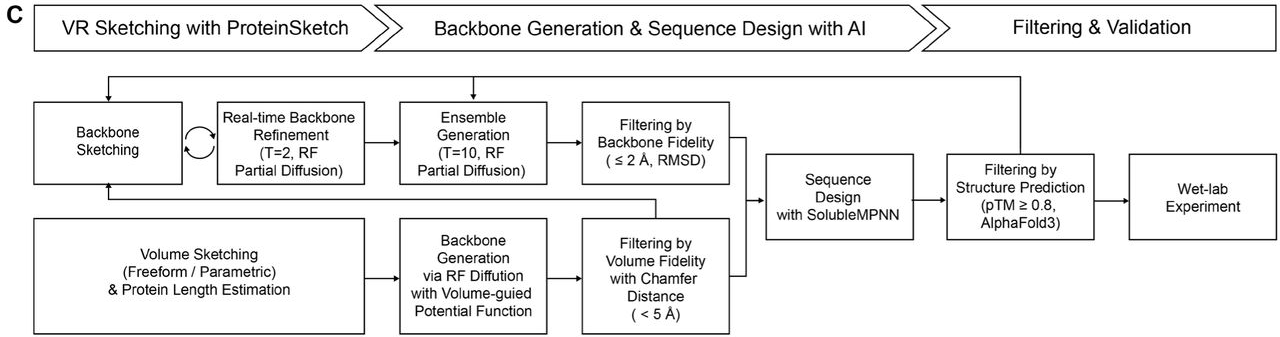
\includegraphics[width=\textwidth]{figures/system-examples/proteinsketch_workflow_crop.png}
  \caption{ProteinSketch connects spatial specification to generative protein design. (A) Two-handed gestures create, reshape, and connect secondary-structure elements in VR. (C) Backbone sketches and volumetric constraints feed computational refinement, generation, sequence design, and filtering. Scientists specify the desired geometry while computational models propose and evaluate candidate structures, linking Immersive and Algorithmic assistance within the design workflow. Selected panels cropped from Ma et al.~\cite{AnchorProteinSketch}, Fig.~1; original panel labels retained.}
  \label{fig:proteinsketch-workflow}
\end{figure*}


Spatial language creates a related requirement: a reference must resolve to identifiable data and an inspectable operation. Section~\ref{sec:modality-vr} contrasts elicited spatial-language requirements with implemented scene operations, keeping both distinct from demonstrated scientific reasoning.


The distinction also limits immersive-assistance claims. Vitessce Link synchronizes selection and other interaction state between mixed-reality and planar clients. Synchronization alone does not establish Immersive assistance, but its hand-controlled measurement tool provides a more specific mechanism: tracked finger positions define endpoints for measuring distances within a tissue map, with applications described for kidney and melanoma structures.~\cite{ExpansionX015} This supports Algorithmic assistance through geometric measurement and a narrowly scoped Immersive placement through embodied specification of that
computation; it does not establish Adaptive assistance or independently validated improvements in analytical performance. Similarly, moleculARweb's implemented SAXS-profile comparison, contact/linker analysis, and constrained molecular mechanics support narrowly scoped analytical functions. ~\cite{ExpansionX012,ExpansionX128}


\subsection{Overlapping Modes and Shifts in Analytic Agency}
\label{sec:assistance-overlap}

Assistance modes combine as analytical work moves between scientists and computational mechanisms. In Facetto, computational organization supports inspection, and expert-provided labels then guide classification. In FathomGPT, linguistic interpretation translates a request into operations whose visual results inform the analyst's next question. In ProteinSketch, scientists express spatial constraints that guide generative computation. Each transition connects a human judgment to a computational contribution and creates an opportunity to inspect the resulting evidence.

Agentic orchestration can plan and coordinate such operations, determining their sequence and how results pass between them. A workflow might combine conversational specification, algorithmic execution, and adaptive suggestions, with distinct opportunities for intervention at each stage. Scientists may revise the initial request, inspect an intermediate result, or redirect a proposed next step. These shifts concern the operational questions in Section~\ref{subsection:locusofagency}: proposal, scope, execution, assessment, and opportunities for inspection and revision. Different participants or computational components can take responsibility for these actions at different points in the workflow.

Clinical registry tools illustrate another division of work. StoryboardR organizes recorded events for visual interpretation, whereas REDCap's generative features can produce a textual summary of report data.~\cite{MillerShalhout2023StoryboardR,Shyr2026REDCapAI} The former delegates presentation; the latter also delegates an interpretive account that the researcher must check. Sections~\ref{sec:modality-desktop} and~\ref{sec:evaluation-effectiveness} examine the interface and evaluation consequences.

These shifts provide a basis for comparing combined assistance: which decisions scientists make directly, which they express through constraints or feedback, and which they delegate to computation. Effective support depends on matching those arrangements to the task and providing ways to inspect and revise consequential outputs. The next section examines how visualization modalities shape these opportunities; Section~\ref{sec:evaluation} considers the evidence needed to establish their analytical benefits.

\section{How Visualization Modality Shapes Assistance}
\label{sec:modality}

Visualization modality conditions how assistance enters an analytical workflow. A recommended selection can appear as a highlighted subset in linked planar views, a region in an immersive volume, or a highlighted area on a shared wall display. Although the computational operation may be similar, the effort needed to specify its target, inspect its consequences, and correct it can differ. Comparing modalities therefore helps explain how an assistance mechanism fits the analyst’s task and working environment.

Building on Section~\ref{sec:assistance}, we examine how each environment shapes the signals available to computational assistance and the ways scientists specify, inspect, and correct analytical operations. The comparison asks which decisions an environment makes accessible, what effort their inspection requires, and how scientists recover when an intervention is inappropriate. This connects the interaction possibilities of each modality to the analytical work they support and to the evaluation conditions needed to assess that support.

Figure~\ref{fig:assistance-modality-map} provides the corresponding system-level map. The following comparisons separate implemented capabilities, reported evaluation, and design implications. Coverage is uneven because the selected evidence supports some task--modality combinations more directly than others; this is not a claim of field-wide absence.


The targeted coverage pass also exposes a distinction between paper-level labels and mechanism-level relationships. A desktop baseline in a VR study does not establish immersive assistance on desktop; CAVE evidence belongs in its separate column. Access remains limiting: reports were unavailable for 86 of 110 Immersive--Desktop system groups, 15 of 20 Immersive--Large Display groups, and 11 of 12 Adaptive--Large Display groups. Unfilled cells therefore cannot be interpreted as combinations that uniformly failed scientific scrutiny.

\subsection{Desktop/Planar Environments}
\label{sec:modality-desktop}

Planar interfaces can place representations, parameters, and explanatory records alongside one another. Precise pointing and text entry support bounded selections and explicit specification, while linked views connect an observation to its surrounding population or evidence. For assisted analysis, these arrangements matter when scientists must inspect what a transformation or recommendation actually changed. Their value depends on the interface making the relevant state available; a desktop display does not guarantee auditability.

The labeling and prediction workflows in Sections~\ref{sec:assistance-adaptive} and~\ref{sec:tasks-comparison} illustrate why co-located views matter: scientists can relate the current selection to model outputs, underlying observations, and source evidence. Their broadly planar setting supports these comparisons, but does not itself guarantee that an intervention is transparent or correct.

StoryboardR provides a clinical-registry example of this arrangement. It transforms REDCap records into patient timelines combining treatment, disease progression, and other clinical events, with hover details available for inspection.~\cite{MillerShalhout2023StoryboardR} The timeline brings temporal relationships into view while clinicians interpret their significance. This example locates computational organization at the presentation stage: assessing additional analytical assistance requires identifying what the system computes beyond preparing and displaying those records.

Conversational execution adds a specification layer rather than replacing inspection. PhenoFlow's request, code, explanation, and field views (Section~\ref{sec:assistance-conversational}) illustrate the need to compare an intended cohort with its generated definition. Such inspectable workflows provide meaningful baselines when spatial interfaces change both representation and input.

\subsection{Large Displays and Collaborative Walls}
\label{sec:modality-walls}

A large display can make several work regions visible while allowing collaborators to pursue different questions. Physical proximity to a region, however, is an ambiguous signal of intent: it may indicate interest, discussion, or simply a convenient position. An adaptive assistant that interprets local activity as a group objective risks turning an individual action into an unintended shared intervention.

Belkacem et al.'s survey of large high-resolution displays identifies the consequences of greater display space and resolution, multiple users, and interaction devices for visualization design.~\cite{belkacem2024large} In assisted life-science analysis, these properties motivate explicit comparison of shared overviews, local work regions, and coordination over computational interventions; display capacity alone does not establish analytical benefit.

Echo offers a life-science example of Algorithmic assistance on a large display: patient summaries and threshold-based anomaly highlighting support ICU handoff discussion.~\cite{MapEcho} Its computational contribution organizes clinical evidence for shared inspection; the display and collaboration do not themselves establish adaptation or improved clinical outcomes.

\emph{Talk to the Wall} illustrates the coexistence of touch and predefined speech commands in collaborative document analysis.~\cite{EvalMolinaLeon2025} Speech makes some operations audible to collaborators and supports interaction from a distance, while recognition errors and distraction complicate coordination. Section~\ref{sec:evaluation-collaboration} examines the study's awareness evidence and its limits; it does not establish autonomous group assistance or improved biological reasoning.

For Coordination and Collaborative Reasoning, the consequential distinction is the scope of a change. In a tissue-analysis scenario, a request to remove low-quality cells might alter one person's view, every linked view, or the group's shared selection. A useful design makes that scope visible before execution, identifies the requester, and permits affected collaborators to inspect or reverse the change. These are design implications, not reported results from the wall study. Shared visibility alone neither records the operation's provenance nor establishes agreement. Evaluation should examine conflicting requests, unnoticed shared changes, and recovery alongside awareness and task performance.

\subsection{Virtual Reality}
\label{sec:modality-vr}

Virtual reality places navigation, spatial reference, and selection within an embodied interaction loop. Assistance may reduce repeated pointing or travel by suggesting a target, changing a viewpoint, or completing a selection. The same intervention can impose reorientation and verification costs. Yang et al.'s comparison of room-sized and zoomable scatterplots, with and without overviews, illustrates the task dependence of navigation costs; it does not isolate an AI-assistance benefit.~\cite{EvalYang2021}

NUI-VR$^2$ and ProteinSketch connect embodied input to different computational responsibilities: specifying segmentation inputs and expressing constraints on generated structures, respectively (Section~\ref{sec:assistance-immersive}). The environmental question is how scientists inspect and correct those inputs in space. A human-performance advantage over planar alternatives would require a comparison of scientists' work in the relevant environments, beyond technical segmentation or design assessments.

Ku\v{t}\'{a}k et al. survey molecular visualization in immersive virtual environments by application area and task, spanning educational uses and scientific workflows such as collaborative drug design.~\cite{kutak2023molecular} This provides domain-specific context for the molecular examples considered here. We additionally distinguish the immersive environment from the implemented computational contribution and from evidence of an advantage for the analyst.

DTBIA couples multiscale brain exploration with filtering and edge bundling in VR.~\cite{MapDTBIA} Its placement connects spatial exploration to computational organization, while its expert cases should not be read as a controlled estimate of an immersive advantage.

SAMIRA extends this comparison to language-mediated segmentation and patient-grounded guidance in VR.~\cite{MapSAMIRA} Its overlapping placements separate execution, context-conditioned guidance, dialogue, and spatial specification; they do not represent four independent systems or four demonstrated effectiveness gains.

VROOM offers a different VR task: inspecting a patient of interest against a cohort through clinical and molecular variables, familiar charts, and similarity-based comparison.~\cite{ExpansionX032} Its value proposition concerns access to comparative evidence within an immersive workspace. That implemented workflow does not by itself establish that spatial context changes the analytical computation, or that immersion improves the resulting clinical interpretation.

Spatial-language examples sharpen this distinction. Song et al.'s Wizard-of-Oz study collected spatial and deictic requests during 3D-scatterplot interaction; researcher-mediated responses reveal interaction requirements, not a validated autonomous resolver.~\cite{SongEmbodiedNLI} VOICE illustrates an implemented conversational molecular-visualization architecture that translates requests into structured operations over a scene model.~\cite{VOICE} It is a mechanism example, not evidence here of a VR-specific analytical advantage. Neither spatial language nor molecular content alone establishes scientific analysis. A request referring to ``those structures'' needs an identifiable target, and a request about interaction partners needs the underlying relationship data rather than a guess from screen-space proximity. Highlighting a proposed referent before a consequential operation can make such ambiguity contestable.

\subsection{Augmented/Mixed Reality}
\label{sec:modality-ar}

Augmented and mixed reality introduce a further relationship to inspect: the alignment between a representation and its physical context. An apparent selection error can arise from registration, occlusion, an unsuitable viewpoint, or a mistaken interpretation of the request. These causes require different remedies. A scientist cannot reliably correct the assistant's reasoning if a displaced overlay is mistaken for an incorrect data relationship.

\begin{figure}[htbp]
\centering
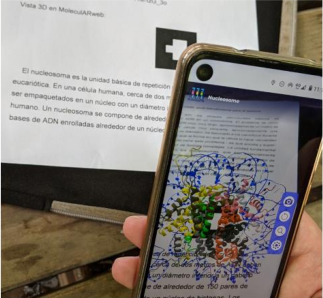
\includegraphics[width=0.72\linewidth]{figures/system-examples/molecularweb_panel_f.pdf}
\caption{moleculARweb displays a molecular model through a smartphone camera view of a printed page containing a fiducial marker. The marker anchors the virtual structure to the physical page, while touch gestures allow the model to be rotated for inspection. This handheld AR configuration combines molecular visualization with a familiar mobile device and printed material. Cropped from Abriata~\cite{Abriata2025MolecularWebUniverse}, Fig.~1(F), licensed under \href{https://creativecommons.org/licenses/by/4.0/}{CC BY 4.0}.}
\label{fig:molecularweb-mobile-ar}
\end{figure}


Francese et al.'s AR application for skin-lesion assessment integrates segmentation, feature extraction, and neural-network classification into an augmented view of the patient's skin.~\cite{MapSkinAR} It connects computed lesion characteristics to the physical target under examination. In a preliminary evaluation with seven dermatologists, six gave positive or very positive feedback on the visualization's usefulness. This provides initial evidence of perceived utility; its effect on diagnostic accuracy and clinical decisions remains to be evaluated.

For Selection, Filtering, and Precision Interaction, a design implication is to expose the selected data identity as well as its spatial highlight. For Comparison and Differentiation, physical placement should not silently substitute for the quantitative or relational basis of the comparison. Adaptive assistance based on position or gaze also needs to distinguish an inferred intention from a confirmed instruction: looking at a structure need not authorize a transformation.

The selected studies motivate these questions but do not establish their resolution through a matched life-science AR/MR evaluation. Registration-aware confirmation, explicit frames of reference, and recovery from misplaced interventions remain requirements to investigate. Findings from planar conversation or VR interaction cannot establish equivalent outcomes in AR/MR, where the environmental conditions differ.

\subsection{CAVE Environments}
\label{sec:modality-cave}

Room-scale projection combines shared physical occupancy with viewpoint-dependent presentation. This changes the coordination problem relative to both a planar wall and individually worn headsets. Where rendering follows one tracked viewpoint, collaborators may not have equivalent views of the same spatial reference. The person issuing a command, the person whose movement informs adaptation, and the people affected by an operation may also differ.

iCAVE supplies an implemented example: network layout, clustering, and edge bundling support biomolecular-network exploration in both desktop and CAVE settings.~\cite{MapICAVE} Figure~\ref{fig:assistance-modality-map} therefore places it under Algorithmic assistance in CAVE. An additional Immersive-assistance placement requires evidence that spatial or embodied context contributes to the analytical computation; that relationship remains unresolved in the assessed report.

ExaViz provides a contrasting CAVE example: molecular navigation and steering connect computed guidance with spatial selection and haptic intervention.~\cite{MapExaViz} Its Adaptive placement rests on target- and geometry-conditioned guidance, while its Immersive placement concerns the coupling to embodied interaction. Neither follows from the CAVE label alone.

For collaborative assistance, a proposed selection or viewpoint change should therefore expose its owner, reference frame, and scope. A recommendation inferred from one participant's behavior should not be interpreted as collective intent. Likewise, a visible shared result does not establish that every participant understood the operation that produced it. These implications connect the signal--inference--intervention account with the distinction between awareness and common ground.

FIESTA's observations of personal and joint work in shared VR provide useful contextual evidence about collaborative workspace organization, but are not a CAVE evaluation.~\cite{EvalLee2021} These findings do not establish improved assisted scientific reasoning in a CAVE environment. A suitable comparison would examine shared reference, competing input, and restoration of context under the actual tracking and rendering configuration, rather than treating all immersive collaboration as interchangeable.

Implemented modality coverage must be checked operation by operation. MinOmics juxtaposes structures on a high-resolution wall and superposes them in a headset for redox-proteomics comparison.~\cite{ExpandedE07} GeneVAnD distributes linked cluster views across a wall, and MDV couples trajectory display with recomputed secondary structure on desktop and a large stereoscopic display.~\cite{ExpandedE06,ExpandedE08} BioNet-XR implements network algorithms on desktop and in VR, but limits its mixed-reality build to importing and navigating networks.~\cite{ExpandedE26} A generic anatomical-model builder's stated CAVE portability likewise does not demonstrate a CAVE workflow.~\cite{ExpandedE01} Platform availability is therefore not evidence that assistance transfers unchanged.

Cross-device workflows combine these environments while requiring continuity of data identity and analytical state. Section~\ref{sec:challenges-continuity} develops those requirements. When studies change display, representation, interaction, and computation together, their results describe a system-level combination rather than an isolated modality effect; Section~\ref{sec:evaluation} addresses the corresponding comparisons.

\section{Evaluation of Assisted Visual Analytics}
\label{sec:evaluation}
Evaluation tests whether a computational contribution helps scientists perform a task and what evidence supports that claim. Isenberg et al.'s review distinguishes goals including computational performance, user performance, and understanding analytical work.~\cite{EvalIsenberg2013} These outcomes are related but not interchangeable. A fast operation can produce an inappropriate comparison; a usable interface can expose a pattern that does not support a biological explanation. The task comparison in Section~\ref{sec:tasks} identifies the accomplishment to assess. The agency questions in Section~\ref{subsection:locusofagency} locate responsibility for proposal, scope, execution, and assessment, and the opportunities to inspect, change, or undo an operation.

The placements in Figure~\ref{fig:assistance-modality-map} establish mechanism--environment relationships, not comparative effectiveness. Each benefit therefore requires evaluation of the task and intervention actually claimed.

The system comparisons identify which contribution an evaluation needs to examine. For a configured pipeline, relevant questions include whether the chosen operations execute correctly and whether their outputs support the intended analysis. When a scientist teaches a classifier through labeled examples, evaluation must also examine how those examples affect subsequent assignments and whether erroneous propagation can be detected and corrected. A generated query requires checking the translation from the scientific request to data and operations, while comparison of supporting evidence requires inspection of provenance, coverage, and disagreement. These requirements follow from the analytical decisions supported or delegated, rather than from a shared interface or assistance label.

\subsection{Analytic Effectiveness and Scientific Utility}
\label{sec:evaluation-effectiveness}
Three checks are needed: whether an operation executes correctly, whether it implements the intended request, and whether its evidence warrants the scientific interpretation. Conversational generation makes the distinction visible: executable code can select the wrong cohort, and a correct cohort comparison may still leave confounding unresolved. For adaptive assistance, prediction accuracy and the benefit of recommending the predicted action require separate evaluation.

The baseline determines which contribution can be isolated. A matched comparison with and without guidance can assess the intervention; changing the display, representation, and interaction simultaneously assesses a system-level combination. Poco et al.'s projection study motivates capable desktop alternatives when evaluating spatial approaches.~\cite{EvalPoco2011} Participant expertise, data complexity, duration, and task definitions must accompany performance results. A prescribed cluster-identification task assesses that bounded accomplishment; the cluster's biological interpretation requires domain evidence.

The RetainVis--MediSyn comparison in Section~\ref{sec:tasks-comparison} illustrates the evidential boundary. Predictive-model measurements and performance on simplified evidence-selection tasks answer different questions. Computational benchmarks establish output properties; controlled studies test bounded human-performance claims; expert cases identify domain relevance; sustained use can reveal effects on an evolving workflow. None should be substituted for another merely because all evaluate the same software.

Operational uptake provides a further kind of evidence. Shyr et al. report REDCap generative-AI use in 958 Vanderbilt projects, including 754 using qualitative summarization and 215 using writing assistance; feature counts overlap.~\cite{Shyr2026REDCapAI} These totals include exploratory and operational use. They establish deployment and use, while summary fidelity, verification effort, and effects on research conclusions require separate assessment. For assisted analysis, a useful next test is whether researchers can identify omissions or unsupported interpretations in generated summaries of their data.

The expanded studies reinforce these distinctions. Interactive AI annotation reports 192 tasks performed by three radiologists, with improved annotation quality for two participants but not the third and concerns about unlocalized model changes.~\cite{ExpandedE24} Five biologists assessing the Space-Time Hypercube found utility for wave detection but mixed results for division and asynchrony tasks.~\cite{ExpandedE22} BioNet-XR's 30-person usability study tested desktop use; immersive versions were presented through videos.~\cite{ExpandedE26} Liver navigation reports phantom registration performance rather than clinical outcomes, and ASCRIBE-XR demonstrates implemented workflows without a user-benefit study.~\cite{ExpandedE15,ExpandedE28} These results cannot be combined into a single claim of analytical effectiveness.

Assessment of metastasis detection for the Augmented Reality Microscope exposes a further complication: agreement with a recorded label need not imply a correct result. Reinspection against immunostains identified discrepancies in the ground truth itself.~\cite{ExpansionX014} Model accuracy, spatial presentation, and assistance to pathological decisions therefore require distinct checks; a detector assessment is not sufficient evidence of improved decision-making through the microscope.

\subsection{Representational Fidelity and Uncertainty}
\label{sec:evaluation-fidelity}
Filtering, aggregation, layout, and embedding change which relationships are available for inspection. Fidelity concerns preservation of the properties needed for the task, rather than a universal preference for maximum detail. Holten's edge bundling reduces clutter while creating ambiguity in following individual edges.~\cite{EvalHolten2006} CMGV's distinction between underlying and visible graphs supports complexity-management operations; integrity and performance tests assess those operations rather than scientists' understanding.~\cite{EvalZafar2026}

Computational and interpretive fidelity require separate evidence. An aggregate may correctly represent a population mean while concealing a small subgroup important to the question. Evaluation can test preservation of relevant structure and whether analysts recognize when omitted detail matters. Biological uncertainty, representational distortion, and uncertainty about intent also need separation. A well-registered spatial highlight may still identify the wrong object; a correct selection may still feed an inappropriate transformation. Combining all three errors into one accuracy measure obscures the correction required.

Useful assessments therefore connect the displayed result to its source observations and active transformations, testing whether scientists can detect a consequential omission, inspect alternatives, and revise an interpretation. The relevant properties depend on the task: orientation requires stable correspondence across scales, while comparison requires a defensible basis for the contrast.

\subsection{Provenance and Recovery}
\label{sec:evaluation-provenance}
Provenance is valuable when scientists can use it to reconstruct and question a result. VisTrails records evolving scientific workflows and supports returning to earlier versions and comparing alternatives.~\cite{EvalFreire2006} This provides a basis for recovery, not proof that a user will notice an error. Conversational explanations add another distinction: an account of what was intended is not evidence of what actually executed. DeepVIS exposes intermediate generation steps and permits targeted refinement, but favorable assessments of inspectability do not establish reliable recovery in biological analysis.~\cite{EvalShuai2025}

Adaptive traces should identify the context and model state used for an intervention, the alternatives shown, and acceptance, rejection, or modification. Subsequent behavior may have been induced by the intervention rather than independently expressing a preference. Reconstruction can require software and model versions, stochastic seeds, parameters, and learned-state updates as well as prompts and outputs.

Recovery should be tested beyond undoing the last action. If an incorrect filter feeds a comparison and generated summary, correcting the filter must also expose stale dependent results. Relevant measures include error detection, localization of the responsible operation, successful restoration or revision, correction time, and persistence of downstream errors. In shared work, the trace also needs to distinguish who proposed, executed, and accepted a change. These checks turn recorded history into usable accountability.

\subsection{Analyst Control, Calibration, and Exploration Bias}
\label{sec:evaluation-control}
Control includes setting assistance scope before an action, accepting or modifying it during execution, and recovering afterward. ProactiveVA users requested finer intervention during agent activity; rapidly changing tasks and noisy traces also complicated intent inference.~\cite{EvalZhao2025} A useful initial suggestion therefore does not establish that later operations remain appropriate.

Calibrated reliance means accepting sound assistance while questioning incorrect or unsupported output. In PhenoFlow, lengthy explanations could conceal errors, while shortening them could remove necessary information; code and data-field inspection provided complementary checks.~\cite{EvalKim2025} Evaluation should measure acceptance of correct suggestions, detection and correction of incorrect ones, and recognition that further evidence is needed. Trust ratings or acceptance frequency alone cannot establish calibration.

Ha et al. compare user models for interaction prediction and exploration-bias detection, separating these capabilities from the benefit of subsequent guidance.~\cite{EvalHa2023} The feedback loop in Section~\ref{sec:assistance-adaptive} motivates following multiple interventions: a recommendation alters the next selection and hence the evidence used to recommend again. Studies can record exposure to alternatives, introduce known intent mismatches, and examine behavior after goals change. Exploration breadth should be interpreted with recognition of contradictory evidence and quality of justification, not rewarded as novelty for its own sake. Expertise in biology, experience with the interface, and familiarity with the model should be reported separately.

\subsection{Workload and Embodied Cost}
\label{sec:evaluation-workload}
Assistance can transfer work from execution to specification, inspection, and repair. Timing only query generation or counting clicks misses the effort required to reach a trustworthy result. Adaptive timing also matters: a correct suggestion may interrupt a demanding comparison. Reorientation, rejected prompts, and explaining changed goals can offset the saved interaction.

Computational delays should be separated by operation. Graphia compares loading, layout, and rendering but notes different layout stopping conditions, limiting direct runtime comparison.~\cite{EvalFreeman2022} Likewise, Yang et al.'s room-sized and zoomable scatterplot conditions reveal task-dependent navigation costs, without isolating an AI contribution.~\cite{EvalYang2021} Assisted viewpoint changes might reduce travel yet increase the effort to recover context.

Selection accuracy, correction actions, task time, and reported effort should therefore be assessed together. Spatial workflows additionally require reporting input devices, seated or standing use, session duration, discomfort, breaks, and withdrawals. Fewer movements may reflect useful computation or inadequate inspection; shorter completion time may coexist with greater mental effort. A practical evaluation follows the entire analytical episode, including waiting, supervision, and recovery.

\subsection{Collaboration and Common Ground}
\label{sec:evaluation-collaboration}
Collaborators need to understand the purpose, state, and evidential basis of shared work. Visibility is only one component. FIESTA's exploratory study of ten groups of three identified movement between personal and joint work and perceived awareness benefits in shared VR.~\cite{EvalLee2021} It did not test autonomous group oversight. In \emph{Talk to the Wall}, ten pairs used speech and touch in document analysis; fourteen participants reported awareness benefits from hearing a partner's commands, while distraction was also a concern.~\cite{EvalMolinaLeon2025} A causal improvement in task speed or accuracy was not demonstrated in that study.

The consequential question is whose intention governs a shared intervention. Following the shared-selection example in Section~\ref{sec:modality-walls}, evaluation should distinguish a private preview from an authorized group change, test whether affected participants notice its scope, and assess whether they can challenge or reverse it. A request from the most active speaker is not evidence of collective agreement.

Relevant outcomes include clarification effort, awareness of consequential changes, resolution of conflicting operations, restoration of prior state, and participants' ability to explain a joint conclusion. Equal command counts are not inherently desirable when roles differ; access to decisions and the ability to contribute or contest evidence matter more. Agreement aids coordination but does not validate a biological claim.

\subsection{Cross-Study Evidence and Limits of Comparability}
\label{sec:evaluation-comparison}
Table~\ref{tab:evaluation-evidence} compares selected evaluations by their intervention, study context, evidence, and limits. It preserves distinctions among computational measurement, controlled task performance, participant feedback, and observations of use. Spatial-language requirements elicited through Wizard-of-Oz methods and implemented scene-operation architectures answer different questions, as discussed in Section~\ref{sec:modality-vr}; neither automatically establishes scientific benefit.

Quantitative comparison is justified when the task, outcome definition, and baseline align. Response time requires equivalent timed work; accuracy requires a comparable target. Where studies are heterogeneous, qualitative comparison can still establish which mechanism was tested and where its evidence stops. Heterogeneity does not justify discarding compatible measurements, and an unevaluated capability is not evidence of failure.

General visualization studies can inform interaction choices without proving biological utility. Domain cases can establish relevance without isolating causal benefit. Across these forms of evidence, the recurring need is to connect the computational contribution to analyst use, error correction, and the scientific judgment that follows. Section~\ref{sec:challenges} develops research directions from those gaps rather than treating greater autonomy or immersion as a goal in itself.
\begin{table*}[t]

\centering

\caption{Selected evaluation examples and the limits of their supported claims. Participant feedback, computational measurements, and observed behavior are identified separately. The comparison concerns the evidence used in this section, rather than every evaluation reported in each paper.}

\label{tab:evaluation-evidence}

\footnotesize

\setlength{\tabcolsep}{4pt}

\renewcommand{\arraystretch}{1.12}

\begin{tabular}{@{}>{\raggedright\arraybackslash}p{.17\textwidth}>{\raggedright\arraybackslash}p{.21\textwidth}>{\raggedright\arraybackslash}p{.24\textwidth}>{\raggedright\arraybackslash}p{.32\textwidth}@{}}

\toprule

\textbf{Study and analytic context} & \textbf{Intervention and comparison} & \textbf{Evidence and study context} & \textbf{Supported claim and limit} \\

\midrule

Graphia~\cite{EvalFreeman2022}: desktop graph exploration & Graph loading, layout, and rendering compared with Gephi and Cytoscape & Computational comparison using three graphs, including a gene-expression graph; hardware and software versions reported & Demonstrates performance characteristics under the tested conditions. Different layout stopping conditions limit runtime comparison; rendering speed does not establish reduced cognitive workload. \\

\addlinespace[3pt]

Yang et al.~\cite{EvalYang2021}: navigation and comparison in VR scatterplots & Room-sized versus zoomable views, each with and without an overview & Controlled comparison of four navigation conditions; task time, accuracy, and navigation analysis & Supports task-dependent navigation choices. It does not isolate an AI intervention or establish biological utility. \\

\addlinespace[3pt]

Ha et al.~\cite{EvalHa2023}: modeling data exploration & Eight user-modeling algorithms compared across four interaction datasets & Computational evaluation of interaction prediction, bias detection, and complexity & Compares user-model performance. Successful prediction or detection does not establish that a subsequent intervention improves exploration. \\

\addlinespace[3pt]

DeepVIS~\cite{EvalShuai2025}: conversational visualization generation & Step-wise generation and editable intermediate decisions; computational baselines and interface evaluation & Generation benchmarks and a 32-participant study; participant assessments of understanding and refinement & Provides distinct evidence about output generation and perceived inspectability. These results do not establish reliable error recovery in biological workflows. \\

\addlinespace[3pt]

PhenoFlow~\cite{EvalKim2025}: clinical cohort exploration & LLM-assisted data wrangling with code, explanation, and data inspection & Design collaboration with two neurologists and clinical case studies; observations during iterative refinement & Grounds inspection requirements in domain practice. Explanation-related difficulties are design evidence, not a controlled estimate of calibration improvement. \\

\addlinespace[3pt]

ProactiveVA~\cite{EvalZhao2025}: proactive assistance during event analysis & Assistance informed by interaction history; comparison with a formative study & Ten-user evaluation with 15-minute exploration, interaction records, ratings, and interviews & Reports use of proactive assistance and identifies steering limitations. A formative-study comparison and short sessions do not establish sustained scientific benefit. \\

\addlinespace[3pt]

FIESTA~\cite{EvalLee2021}: collaborative analysis in a shared VR workspace & Configurations supporting individual and joint work & Exploratory study with ten groups of three using housing data; behavior observations and participant feedback & Identifies coordination practices and perceived awareness benefits. Timing differences were not strictly controlled; autonomous group oversight was not tested. \\

\addlinespace[3pt]

Talk to the Wall~\cite{EvalMolinaLeon2025}: collaborative analysis on a large display & Speech and touch used within a shared workspace & Ten-pair study; interaction records and participant reports & Shows how speech can make actions available to collaborators while raising distraction concerns. Positive reports do not establish a causal gain in team accuracy or autonomous oversight. \\

\bottomrule

\end{tabular}

\end{table*}

\section{Research Challenges and Opportunities}
\label{sec:challenges}
The comparisons in Sections~\ref{sec:tasks}--\ref{sec:evaluation} identify recurring questions about the decisions scientists retain, the transformations they must inspect, and the evidence supporting an interpretation. Feedback-driven classification raises questions about correction and propagated changes; generated operations raise questions about intent and execution provenance; shared and spatial workflows raise questions about authority, reference, and continuity. The following agenda develops these differences into design opportunities and testable questions concerning revisable delegation, inspectable transformations, traceable evidence, collaborative common ground, and continuity across environments.

The expanded cases make transformation risks concrete. Space-Time Hypercube projection can obscure spatial information and create apparent shrinkage as objects move away from a cutting plane; source-geometry views provide a partial safeguard.~\cite{ExpandedE22} PathwayMatrix's binary decomposition supports overview while limiting temporal and causal tracing.~\cite{ExpandedE37} Such trade-offs motivate preservation of source links and transformation assumptions, not rejection of computational abstraction.

\subsection{Delegation and Analyst Control}
\label{sec:challenges-delegation}
Delegated work must remain revisable when a scientist changes a question or discovers a problem. Approving an initial plan does not necessarily provide control over its later consequences. ProactiveVA illustrates this distinction: adjustable guidance frequency did not resolve a participant's request to intervene while an agent was executing.~\cite{EvalZhao2025} As Section~\ref{sec:evaluation-control} explains, control over assistance appearing and control over its execution are different capabilities.

A useful direction is to represent delegated work through explicit inputs, constraints, dependencies, and intervention points. If a scientist changes a cohort after inspecting a heatmap, the system should identify affected comparisons while preserving valid intermediate results. Routine recomputation under established parameters need not require the same supervision as changing the population or ranking criterion. Adaptive systems must additionally distinguish an inferred preference from permission to act; uncertainty and reversibility should influence whether to execute, clarify, or refrain.

Institutional deployment adds another level of control. REDCap's generative features are enabled by administrators through an institution-managed AI connection, with user permissions and researcher review of outputs; the underlying research data remain unchanged.~\cite{Shyr2026REDCapAI} This separates authority to enable a capability from responsibility for accepting its result. An analytical workflow should make both decisions visible and preserve links from an accepted summary to the records and request supporting it. The uptake evidence is discussed in Section~\ref{sec:evaluation-effectiveness}.

Studies should introduce changing goals during Selection, Filtering, and Precision Interaction and Comparison and Differentiation. Comparing whole-plan approval, operation-level approval, and consequential checkpoints would reveal whether analysts detect mismatches, redirect work, and preserve valid results. Total specification, supervision, and recovery effort matters more than the number of automated steps.

\subsection{Compression and Representational Fidelity}
\label{sec:challenges-compression}
Filtering, aggregation, and approximation make large datasets tractable while changing which relationships remain visible. The edge-tracing ambiguity discussed in Section~\ref{sec:evaluation-fidelity} illustrates why a clearer overview does not guarantee reliable detailed interpretation.~\cite{EvalHolten2006} Additional display space cannot recover evidence already removed from a representation.

A promising design direction connects summaries to their contributing observations and transformation choices, while indicating where reduction may matter. A heatmap of cell-group averages could expose group size and within-group variation so that a similar average does not silently conceal divergent responses. Access to detail is necessary but may be insufficient if the scientist has no reason to inspect the affected group. Adaptive aggregation also needs visible scope: a display change can reflect a changed representation rather than changed biology.

For Navigation and Multiscale Orientation and Comparison and Differentiation, evaluations should combine broad patterns with localized exceptions. Compare fixed summaries, expandable summaries, and summaries that indicate potentially obscured variation. Measure detection of exceptions, attribution of representational effects, and revision of conclusions when detail contradicts the overview. Compression succeeds scientifically when analysts can discover when omitted detail matters.

\subsection{Guidance and Diversity of Exploration}
\label{sec:challenges-guidance}
Predicting the analyst's next action is different from improving the inquiry, as the user-model comparison in Section~\ref{sec:evaluation-control} makes clear.~\cite{EvalHa2023} Guidance can reinforce familiar variables and explanations; the resulting interactions can then become evidence for further recommendations. Apparent preference stability may partly reflect the system's own influence.

Research should distinguish suggestions that extend an analysis, test its robustness, or examine competing explanations. In an expression study, recommending more genes with similar profiles can deepen one pattern without distinguishing treatment response from cell-composition differences. Matched-population comparisons or quality checks may offer more consequential alternatives. These purposes are interaction choices within existing assistance modes, not new taxonomy categories.

Systems could record whether feedback was volunteered or elicited by a suggestion and allow analysts to revise or suspend inferred preferences. Evaluations should assess recognition of conflicting evidence and justification of conclusions alongside coverage and effort. Focused exploration is not inherently biased, and more diverse exploration is not automatically better: the relevant question is whether assistance helps scientists recognize when their evidence warrants another direction.

\subsection{Generative Capability and Scientific Provenance}
\label{sec:challenges-generative}
Generated queries, code, views, and explanations introduce linked interpretive choices. Section~\ref{sec:evaluation-provenance} distinguishes a fluent account from an execution record; the PhenoFlow example also shows that correct execution cannot supply information absent from the data.~\cite{EvalKim2025} A revised question should retain the missing evidence or assumption that motivated the revision.

The research opportunity is to connect requests, plans, executed operations, results, and interpretations while recording their evidential status. CausalChat distinguishes suggested links from data-confirmed relationships; planning systems such as LightVA introduce dependencies through which an upstream revision can undermine later reasoning even if code still executes.~\cite{CausalChat,LightVA} These contextual examples motivate requirements rather than establish solutions for life-science practice.

A generated biological explanation should distinguish an observed difference, the comparison producing it, supporting literature, and the proposed mechanism. Changes to the comparison should identify dependent statements requiring reassessment. Studies can introduce unavailable variables, misleading explanations, execution discrepancies, and stale claims to test whether scientists locate the problem and correct it. Spoken or spatially presented assistance needs the same persistent route to evidence as a desktop explanation.

\subsection{Personalization and Collaborative Common Ground}
\label{sec:challenges-personalization}
Personalization can support different expertise while concealing differences in assumptions. The awareness--distraction tension in \emph{Talk to the Wall} motivates a related question: which consequential changes should collaborators see, and when?~\cite{EvalMolinaLeon2025} Its speech findings do not themselves validate personalized assistance; Section~\ref{sec:evaluation-collaboration} preserves that boundary.

Consider a biologist receiving population suggestions while a computational analyst receives normalization guidance. Private exploration may be useful, but changing a shared heatmap's underlying observations requires common awareness of the filter, its consequences, and whether the change has been adopted. Broadcasting every suggestion is unnecessary; silently changing shared evidence is unsafe for interpretation.

A useful direction supports transitions from private previews to attributed proposals and reversible shared changes. Permission to display a recommendation differs from permission to retrain a common model or publish a joint interpretation. Acceptance by the most active speaker should not imply collective agreement. Studies spanning separate and joint work should measure recognition of divergent assumptions, conflict resolution, participation, interruption costs, and the team's ability to explain a shared conclusion.

\subsection{Modality Specialization and Workflow Continuity}
\label{sec:challenges-continuity}
\label{sec:modality-continuity}
Moving between desktop, immersive, and shared environments should preserve object identities, selection criteria, transformations, uncertainty, and decision history while adapting controls to each setting. These workflows combine existing modalities. Navigation requires recovering context; selection preserves the intended subset; comparison preserves its basis; sensemaking traces evidence; collaboration makes consequential changes intelligible to others.

DashSpace provides an architectural example of cross-device synchronization while leaving semantic conflicts open.~\cite{AgendaBorowski2025} A tissue region selected in VR must refer to the same observations in a desktop matrix; a request about ``these cells'' needs a recorded referent. Spatial-language requirements and implemented scene operations provide complementary starting points.~\cite{SongEmbodiedNLI,VOICE} Research should expose ambiguity, invalidate stale references, and make changes to shared analysis attributable and reversible.

Preferences inferred in one setting should not silently govern a different task. Accessible alternatives should permit inspection and correction without a headset or particular input method. Studies should follow complete transitions, examining reorientation, stale-state detection, correction, and participation, and tracking who proposes, scopes, performs, and assesses consequential operations.

\subsection{Shared Scenarios and Analytical Traces}
\label{sec:challenges-evaluation}
Shared life-science scenarios and analytical traces could support the evaluations developed in Section~\ref{sec:evaluation}. Domain experts should document plausible questions, alternatives, errors, and recovery paths, including inappropriate filters, contradictory evidence, and changing goals. Traces should connect requests, data versions, parameters, transformations, outputs, and revisions, recording who proposed, scoped, performed, and assessed each operation and the opportunities to inspect, change, or undo it. Shared definitions, trace schemas, and permitted data or synthetic substitutes would allow assistance ablations and matched workflow studies to reuse comparable conditions while accommodating several defensible conclusions in open-ended inquiry.

\section{Conclusion}
\label{sec:conclusion}
AI-assisted visual analytics derives its value from the computational contribution to a scientific task and the judgments scientists can inspect and revise. Similar interfaces can distribute work differently: configuring a pipeline differs from teaching a model, and manipulating a representation differs from specifying a generative constraint.

The three perspectives work together as a map, a lens, and a light. The Assistance $\times$ Visualization Modality map locates approaches, the task lens makes their analytical purposes comparable, and the light of analytic agency reveals how consequential choices are distributed between scientists and computation. Read together, these perspectives shift attention from the presence of AI or an immersive interface to the work a mechanism enables, the judgments it influences, and the opportunities it leaves for inspection and correction. The central question is how a particular division of work supports a scientific purpose, and what evidence establishes that support. Progress from hairballs to hypotheses is meaningful when scientists can explain not only what an assisted analysis suggests, but why its evidence warrants the next question.

\label{main-text-end}
\clearpage
\bibliographystyle{eg-alpha-doi}
\bibliography{references}
\end{document}
